\documentclass[1p]{elsarticle_modified}
%\bibliographystyle{elsarticle-num}

%\usepackage[colorlinks]{hyperref}
%\usepackage{abbrmath_seonhwa} %\Abb, \Ascr, \Acal ,\Abf, \Afrak
\usepackage{amsfonts}
\usepackage{amssymb}
\usepackage{amsmath}
\usepackage{amsthm}
\usepackage{scalefnt}
\usepackage{amsbsy}
\usepackage{kotex}
\usepackage{caption}
\usepackage{subfig}
\usepackage{color}
\usepackage{graphicx}
\usepackage{xcolor} %% white, black, red, green, blue, cyan, magenta, yellow
\usepackage{float}
\usepackage{setspace}
\usepackage{hyperref}

\usepackage{tikz}
\usetikzlibrary{arrows}

\usepackage{multirow}
\usepackage{array} % fixed length table
\usepackage{hhline}

%%%%%%%%%%%%%%%%%%%%%
\makeatletter
\renewcommand*\env@matrix[1][\arraystretch]{%
	\edef\arraystretch{#1}%
	\hskip -\arraycolsep
	\let\@ifnextchar\new@ifnextchar
	\array{*\c@MaxMatrixCols c}}
\makeatother %https://tex.stackexchange.com/questions/14071/how-can-i-increase-the-line-spacing-in-a-matrix
%%%%%%%%%%%%%%%

\usepackage[normalem]{ulem}

\newcommand{\msout}[1]{\ifmmode\text{\sout{\ensuremath{#1}}}\else\sout{#1}\fi}
%SOURCE: \msout is \stkout macro in https://tex.stackexchange.com/questions/20609/strikeout-in-math-mode

\newcommand{\cancel}[1]{
	\ifmmode
	{\color{red}\msout{#1}}
	\else
	{\color{red}\sout{#1}}
	\fi
}

\newcommand{\add}[1]{
	{\color{blue}\uwave{#1}}
}

\newcommand{\replace}[2]{
	\ifmmode
	{\color{red}\msout{#1}}{\color{blue}\uwave{#2}}
	\else
	{\color{red}\sout{#1}}{\color{blue}\uwave{#2}}
	\fi
}

\newcommand{\Sol}{\mathcal{S}} %segment
\newcommand{\D}{D} %diagram
\newcommand{\A}{\mathcal{A}} %arc


%%%%%%%%%%%%%%%%%%%%%%%%%%%%%5 test

\def\sl{\operatorname{\textup{SL}}(2,\Cbb)}
\def\psl{\operatorname{\textup{PSL}}(2,\Cbb)}
\def\quan{\mkern 1mu \triangleright \mkern 1mu}

\theoremstyle{definition}
\newtheorem{thm}{Theorem}[section]
\newtheorem{prop}[thm]{Proposition}
\newtheorem{lem}[thm]{Lemma}
\newtheorem{ques}[thm]{Question}
\newtheorem{cor}[thm]{Corollary}
\newtheorem{defn}[thm]{Definition}
\newtheorem{exam}[thm]{Example}
\newtheorem{rmk}[thm]{Remark}
\newtheorem{alg}[thm]{Algorithm}

\newcommand{\I}{\sqrt{-1}}
\begin{document}

%\begin{frontmatter}
%
%\title{Boundary parabolic representations of knots up to 8 crossings}
%
%%% Group authors per affiliation:
%\author{Yunhi Cho} 
%\address{Department of Mathematics, University of Seoul, Seoul, Korea}
%\ead{yhcho@uos.ac.kr}
%
%
%\author{Seonhwa Kim} %\fnref{s_kim}}
%\address{Center for Geometry and Physics, Institute for Basic Science, Pohang, 37673, Korea}
%\ead{ryeona17@ibs.re.kr}
%
%\author{Hyuk Kim}
%\address{Department of Mathematical Sciences, Seoul National University, Seoul 08826, Korea}
%\ead{hyukkim@snu.ac.kr}
%
%\author{Seokbeom Yoon}
%\address{Department of Mathematical Sciences, Seoul National University, Seoul, 08826,  Korea}
%\ead{sbyoon15@snu.ac.kr}
%
%\begin{abstract}
%We find all boundary parabolic representation of knots up to 8 crossings.
%
%\end{abstract}
%\begin{keyword}
%    \MSC[2010] 57M25 
%\end{keyword}
%
%\end{frontmatter}

%\linenumbers
%\tableofcontents
%
\newcommand\colored[1]{\textcolor{white}{\rule[-0.35ex]{0.8em}{1.4ex}}\kern-0.8em\color{red} #1}%
%\newcommand\colored[1]{\textcolor{white}{ #1}\kern-2.17ex	\textcolor{white}{ #1}\kern-1.81ex	\textcolor{white}{ #1}\kern-2.15ex\color{red}#1	}

{\Large $\underline{12a_{0209}~(K12a_{0209})}$}

\setlength{\tabcolsep}{10pt}
\renewcommand{\arraystretch}{1.6}
\vspace{1cm}\begin{tabular}{m{100pt}>{\centering\arraybackslash}m{274pt}}
\multirow{5}{120pt}{
	\centering
	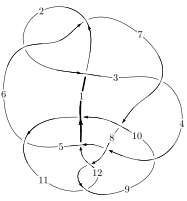
\includegraphics[width=112pt]{../../../GIT/diagram.site/Diagrams/png/1010_12a_0209.png}\\
\ \ \ A knot diagram\footnotemark}&
\allowdisplaybreaks
\textbf{Linearized knot diagam} \\
\cline{2-2}
 &
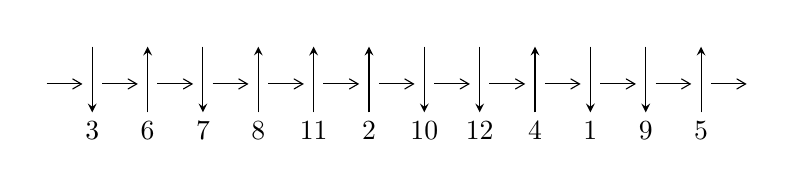
\begin{tikzpicture}[x=20pt, y=17pt]
	% nodes
	\node (C0) at (0, 0) {};
	\node (C1) at (1, 0) {};
	\node (C1U) at (1, +1) {};
	\node (C1D) at (1, -1) {3};

	\node (C2) at (2, 0) {};
	\node (C2U) at (2, +1) {};
	\node (C2D) at (2, -1) {6};

	\node (C3) at (3, 0) {};
	\node (C3U) at (3, +1) {};
	\node (C3D) at (3, -1) {7};

	\node (C4) at (4, 0) {};
	\node (C4U) at (4, +1) {};
	\node (C4D) at (4, -1) {8};

	\node (C5) at (5, 0) {};
	\node (C5U) at (5, +1) {};
	\node (C5D) at (5, -1) {11};

	\node (C6) at (6, 0) {};
	\node (C6U) at (6, +1) {};
	\node (C6D) at (6, -1) {2};

	\node (C7) at (7, 0) {};
	\node (C7U) at (7, +1) {};
	\node (C7D) at (7, -1) {10};

	\node (C8) at (8, 0) {};
	\node (C8U) at (8, +1) {};
	\node (C8D) at (8, -1) {12};

	\node (C9) at (9, 0) {};
	\node (C9U) at (9, +1) {};
	\node (C9D) at (9, -1) {4};

	\node (C10) at (10, 0) {};
	\node (C10U) at (10, +1) {};
	\node (C10D) at (10, -1) {1};

	\node (C11) at (11, 0) {};
	\node (C11U) at (11, +1) {};
	\node (C11D) at (11, -1) {9};

	\node (C12) at (12, 0) {};
	\node (C12U) at (12, +1) {};
	\node (C12D) at (12, -1) {5};
	\node (C13) at (13, 0) {};

	% arrows
	\draw[->,>={angle 60}]
	(C0) edge (C1) (C1) edge (C2) (C2) edge (C3) (C3) edge (C4) (C4) edge (C5) (C5) edge (C6) (C6) edge (C7) (C7) edge (C8) (C8) edge (C9) (C9) edge (C10) (C10) edge (C11) (C11) edge (C12) (C12) edge (C13) ;	\draw[->,>=stealth]
	(C1U) edge (C1D) (C2D) edge (C2U) (C3U) edge (C3D) (C4D) edge (C4U) (C5D) edge (C5U) (C6D) edge (C6U) (C7U) edge (C7D) (C8U) edge (C8D) (C9D) edge (C9U) (C10U) edge (C10D) (C11U) edge (C11D) (C12D) edge (C12U) ;
	\end{tikzpicture} \\
\hhline{~~} \\& 
\textbf{Solving Sequence} \\ \cline{2-2} 
 &
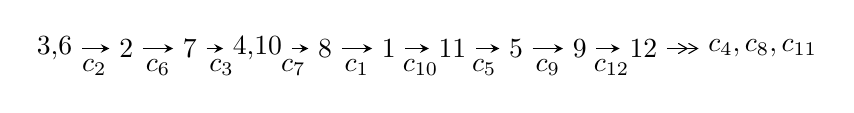
\begin{tikzpicture}[x=23pt, y=7pt]
	% node
	\node (A0) at (-1/8, 0) {3,6};
	\node (A1) at (1, 0) {2};
	\node (A2) at (2, 0) {7};
	\node (A3) at (49/16, 0) {4,10};
	\node (A4) at (33/8, 0) {8};
	\node (A5) at (41/8, 0) {1};
	\node (A6) at (49/8, 0) {11};
	\node (A7) at (57/8, 0) {5};
	\node (A8) at (65/8, 0) {9};
	\node (A9) at (73/8, 0) {12};
	\node (C1) at (1/2, -1) {$c_{2}$};
	\node (C2) at (3/2, -1) {$c_{6}$};
	\node (C3) at (5/2, -1) {$c_{3}$};
	\node (C4) at (29/8, -1) {$c_{7}$};
	\node (C5) at (37/8, -1) {$c_{1}$};
	\node (C6) at (45/8, -1) {$c_{10}$};
	\node (C7) at (53/8, -1) {$c_{5}$};
	\node (C8) at (61/8, -1) {$c_{9}$};
	\node (C9) at (69/8, -1) {$c_{12}$};
	\node (A10) at (11, 0) {$c_{4},c_{8},c_{11}$};

	% edge
	\draw[->,>=stealth]	
	(A0) edge (A1) (A1) edge (A2) (A2) edge (A3) (A3) edge (A4) (A4) edge (A5) (A5) edge (A6) (A6) edge (A7) (A7) edge (A8) (A8) edge (A9) ;
	\draw[->>,>={angle 60}]	
	(A9) edge (A10);
\end{tikzpicture} \\ 

\end{tabular} \\

\footnotetext{
The image of knot diagram is generated by the software ``\textbf{Draw programme}" developed by Andrew Bartholomew(\url{http://www.layer8.co.uk/maths/draw/index.htm\#Running-draw}), where we modified some parts for our purpose(\url{https://github.com/CATsTAILs/LinksPainter}).
}\phantom \\ \newline 
\centering \textbf{Ideals for irreducible components\footnotemark of $X_{\text{par}}$} 
 
\begin{align*}
I^u_{1}&=\langle 
-1.56131\times10^{18} u^{72}+4.31036\times10^{18} u^{71}+\cdots+2.30896\times10^{17} b+2.90849\times10^{19},\\
\phantom{I^u_{1}}&\phantom{= \langle  }2.90849\times10^{19} u^{72}+2.93972\times10^{20} u^{71}+\cdots+4.61791\times10^{17} a+5.31033\times10^{19},\;u^{73}+10 u^{72}+\cdots+17 u+2\rangle \\
I^u_{2}&=\langle 
9 u^{48}-22 u^{47}+\cdots+2 b+2,\;2 u^{48} a+4 u^{48}+\cdots-15 a-7,\;u^{49}-3 u^{48}+\cdots-3 u+1\rangle \\
I^u_{3}&=\langle 
2 u^{26}-22 u^{25}+\cdots+b+16,\;16 u^{26}-46 u^{25}+\cdots+a+9,\;u^{27}-3 u^{26}+\cdots+5 u-1\rangle \\
I^u_{4}&=\langle 
a^3 u+a^3- a^2 u- a^2+b- a- u+1,\;a^4+a^2 u- a^2-2 a u-2 a-2 u-2,\;u^2+u+1\rangle \\
\\
\end{align*}
\raggedright * 4 irreducible components of $\dim_{\mathbb{C}}=0$, with total 206 representations.\\
\footnotetext{All coefficients of polynomials are rational numbers. But the coefficients are sometimes approximated in decimal forms when there is not enough margin.}
\newpage
\renewcommand{\arraystretch}{1}
\centering \section*{I. $I^u_{1}= \langle -1.56\times10^{18} u^{72}+4.31\times10^{18} u^{71}+\cdots+2.31\times10^{17} b+2.91\times10^{19},\;2.91\times10^{19} u^{72}+2.94\times10^{20} u^{71}+\cdots+4.62\times10^{17} a+5.31\times10^{19},\;u^{73}+10 u^{72}+\cdots+17 u+2 \rangle$}
\flushleft \textbf{(i) Arc colorings}\\
\begin{tabular}{m{7pt} m{180pt} m{7pt} m{180pt} }
\flushright $a_{3}=$&$\begin{pmatrix}1\\0\end{pmatrix}$ \\
\flushright $a_{6}=$&$\begin{pmatrix}0\\u\end{pmatrix}$ \\
\flushright $a_{2}=$&$\begin{pmatrix}1\\u^2\end{pmatrix}$ \\
\flushright $a_{7}=$&$\begin{pmatrix}u\\u^3+u\end{pmatrix}$ \\
\flushright $a_{4}=$&$\begin{pmatrix}u^4+u^2+1\\u^6+2 u^4+u^2\end{pmatrix}$ \\
\flushright $a_{10}=$&$\begin{pmatrix}-62.9827 u^{72}-636.589 u^{71}+\cdots-948.579 u-114.994\\6.76197 u^{72}-18.6680 u^{71}+\cdots-955.713 u-125.965\end{pmatrix}$ \\
\flushright $a_{8}=$&$\begin{pmatrix}44.3628 u^{72}+426.580 u^{71}+\cdots+440.294 u+50.3153\\17.0477 u^{72}+207.544 u^{71}+\cdots+704.852 u+88.7256\end{pmatrix}$ \\
\flushright $a_{1}=$&$\begin{pmatrix}u^2+1\\u^2\end{pmatrix}$ \\
\flushright $a_{11}=$&$\begin{pmatrix}-12.7540 u^{72}-143.072 u^{71}+\cdots-330.334 u-40.7974\\38.5297 u^{72}+343.881 u^{71}+\cdots-80.7329 u-18.6829\end{pmatrix}$ \\
\flushright $a_{5}=$&$\begin{pmatrix}-18.2285 u^{72}-181.746 u^{71}+\cdots-197.107 u-22.7670\\9.87004 u^{72}+61.1843 u^{71}+\cdots-257.594 u-34.4057\end{pmatrix}$ \\
\flushright $a_{9}=$&$\begin{pmatrix}-28.7372 u^{72}-293.466 u^{71}+\cdots-456.109 u-56.4533\\17.1086 u^{72}+131.737 u^{71}+\cdots-229.536 u-33.0173\end{pmatrix}$ \\
\flushright $a_{12}=$&$\begin{pmatrix}1.86084 u^{72}+5.66695 u^{71}+\cdots-39.3331 u-0.499919\\33.5377 u^{72}+304.934 u^{71}+\cdots+28.0721 u-1.32706\end{pmatrix}$\\&\end{tabular}
\flushleft \textbf{(ii) Obstruction class $= -1$}\\~\\
\flushleft \textbf{(iii) Cusp Shapes $= -\frac{31874848749235508694}{230895744813749827} u^{72}-\frac{257490262863303824255}{230895744813749827} u^{71}+\cdots+\frac{54578403100783767899}{230895744813749827} u+\frac{6305572019569292940}{230895744813749827}$}\\~\\
\newpage\renewcommand{\arraystretch}{1}
\flushleft \textbf{(iv) u-Polynomials at the component}\newline \\
\begin{tabular}{m{50pt}|m{274pt}}
Crossings & \hspace{64pt}u-Polynomials at each crossing \\
\hline $$\begin{aligned}c_{1}\end{aligned}$$&$\begin{aligned}
&u^{73}+38 u^{72}+\cdots-23 u-4
\end{aligned}$\\
\hline $$\begin{aligned}c_{2},c_{6}\end{aligned}$$&$\begin{aligned}
&u^{73}-10 u^{72}+\cdots+17 u-2
\end{aligned}$\\
\hline $$\begin{aligned}c_{3}\end{aligned}$$&$\begin{aligned}
&u^{73}+10 u^{72}+\cdots-130207 u-16754
\end{aligned}$\\
\hline $$\begin{aligned}c_{4},c_{12}\end{aligned}$$&$\begin{aligned}
&u^{73}+2 u^{72}+\cdots+u+1
\end{aligned}$\\
\hline $$\begin{aligned}c_{5},c_{9}\end{aligned}$$&$\begin{aligned}
&u^{73}+7 u^{71}+\cdots+19 u+7
\end{aligned}$\\
\hline $$\begin{aligned}c_{7},c_{10}\end{aligned}$$&$\begin{aligned}
&u^{73}-3 u^{72}+\cdots-6 u+1
\end{aligned}$\\
\hline $$\begin{aligned}c_{8},c_{11}\end{aligned}$$&$\begin{aligned}
&u^{73}-17 u^{72}+\cdots-4311 u+160
\end{aligned}$\\
\hline
\end{tabular}\\~\\
\newpage\renewcommand{\arraystretch}{1}
\flushleft \textbf{(v) Riley Polynomials at the component}\newline \\
\begin{tabular}{m{50pt}|m{274pt}}
Crossings & \hspace{64pt}Riley Polynomials at each crossing \\
\hline $$\begin{aligned}c_{1}\end{aligned}$$&$\begin{aligned}
&y^{73}-2 y^{72}+\cdots+241 y-16
\end{aligned}$\\
\hline $$\begin{aligned}c_{2},c_{6}\end{aligned}$$&$\begin{aligned}
&y^{73}+38 y^{72}+\cdots-23 y-4
\end{aligned}$\\
\hline $$\begin{aligned}c_{3}\end{aligned}$$&$\begin{aligned}
&y^{73}-36 y^{72}+\cdots-3279540855 y-280696516
\end{aligned}$\\
\hline $$\begin{aligned}c_{4},c_{12}\end{aligned}$$&$\begin{aligned}
&y^{73}-54 y^{72}+\cdots+127 y-1
\end{aligned}$\\
\hline $$\begin{aligned}c_{5},c_{9}\end{aligned}$$&$\begin{aligned}
&y^{73}+14 y^{72}+\cdots-1389 y-49
\end{aligned}$\\
\hline $$\begin{aligned}c_{7},c_{10}\end{aligned}$$&$\begin{aligned}
&y^{73}+21 y^{72}+\cdots-48 y-1
\end{aligned}$\\
\hline $$\begin{aligned}c_{8},c_{11}\end{aligned}$$&$\begin{aligned}
&y^{73}+37 y^{72}+\cdots+996881 y-25600
\end{aligned}$\\
\hline
\end{tabular}\\~\\
\newpage\flushleft \textbf{(vi) Complex Volumes and Cusp Shapes}
$$\begin{array}{c|c|c}  
\text{Solutions to }I^u_{1}& \I (\text{vol} + \sqrt{-1}CS) & \text{Cusp shape}\\
 \hline 
\begin{aligned}
u &= \phantom{-}0.564959 + 0.847230 I \\
a &= -0.420644 + 0.433873 I \\
b &= \phantom{-}0.605237 + 0.111262 I\end{aligned}
 & \phantom{-}6.48655 + 2.06213 I & \phantom{-0.000000 } 0 \\ \hline\begin{aligned}
u &= \phantom{-}0.564959 - 0.847230 I \\
a &= -0.420644 - 0.433873 I \\
b &= \phantom{-}0.605237 - 0.111262 I\end{aligned}
 & \phantom{-}6.48655 - 2.06213 I & \phantom{-0.000000 } 0 \\ \hline\begin{aligned}
u &= -0.372313 + 0.889151 I \\
a &= \phantom{-}1.274400 + 0.272841 I \\
b &= \phantom{-}0.717072 - 1.031550 I\end{aligned}
 & \phantom{-}1.56727 - 2.14796 I & \phantom{-0.000000 } 0 \\ \hline\begin{aligned}
u &= -0.372313 - 0.889151 I \\
a &= \phantom{-}1.274400 - 0.272841 I \\
b &= \phantom{-}0.717072 + 1.031550 I\end{aligned}
 & \phantom{-}1.56727 + 2.14796 I & \phantom{-0.000000 } 0 \\ \hline\begin{aligned}
u &= \phantom{-}0.623366 + 0.835016 I \\
a &= -0.536860 - 0.095790 I \\
b &= \phantom{-}0.254674 + 0.507999 I\end{aligned}
 & \phantom{-}2.20061 + 7.49260 I & \phantom{-0.000000 } 0 \\ \hline\begin{aligned}
u &= \phantom{-}0.623366 - 0.835016 I \\
a &= -0.536860 + 0.095790 I \\
b &= \phantom{-}0.254674 - 0.507999 I\end{aligned}
 & \phantom{-}2.20061 - 7.49260 I & \phantom{-0.000000 } 0 \\ \hline\begin{aligned}
u &= -0.951897 + 0.435766 I \\
a &= -0.211932 + 0.335549 I \\
b &= -0.055516 + 0.411761 I\end{aligned}
 & \phantom{-}3.57693 - 3.95252 I & \phantom{-0.000000 } 0 \\ \hline\begin{aligned}
u &= -0.951897 - 0.435766 I \\
a &= -0.211932 - 0.335549 I \\
b &= -0.055516 - 0.411761 I\end{aligned}
 & \phantom{-}3.57693 + 3.95252 I & \phantom{-0.000000 } 0 \\ \hline\begin{aligned}
u &= \phantom{-}0.640065 + 0.697540 I \\
a &= \phantom{-}0.461939 - 0.202848 I \\
b &= -0.437165 - 0.192384 I\end{aligned}
 & \phantom{-}2.58609 - 2.60921 I & \phantom{-0.000000 } 0 \\ \hline\begin{aligned}
u &= \phantom{-}0.640065 - 0.697540 I \\
a &= \phantom{-}0.461939 + 0.202848 I \\
b &= -0.437165 + 0.192384 I\end{aligned}
 & \phantom{-}2.58609 + 2.60921 I & \phantom{-0.000000 } 0\\
 \hline 
 \end{array}$$\newpage$$\begin{array}{c|c|c}  
\text{Solutions to }I^u_{1}& \I (\text{vol} + \sqrt{-1}CS) & \text{Cusp shape}\\
 \hline 
\begin{aligned}
u &= \phantom{-}0.735332 + 0.754639 I \\
a &= -0.331872 + 0.216445 I \\
b &= \phantom{-}0.407374 + 0.091284 I\end{aligned}
 & \phantom{-}6.04236 - 7.53790 I & \phantom{-0.000000 } 0 \\ \hline\begin{aligned}
u &= \phantom{-}0.735332 - 0.754639 I \\
a &= -0.331872 - 0.216445 I \\
b &= \phantom{-}0.407374 - 0.091284 I\end{aligned}
 & \phantom{-}6.04236 + 7.53790 I & \phantom{-0.000000 } 0 \\ \hline\begin{aligned}
u &= \phantom{-}0.584696 + 0.704579 I \\
a &= \phantom{-}0.677743 + 0.287959 I \\
b &= -0.193384 - 0.645892 I\end{aligned}
 & \phantom{-}6.89806 + 2.50124 I & \phantom{-0.000000 } 0 \\ \hline\begin{aligned}
u &= \phantom{-}0.584696 - 0.704579 I \\
a &= \phantom{-}0.677743 - 0.287959 I \\
b &= -0.193384 + 0.645892 I\end{aligned}
 & \phantom{-}6.89806 - 2.50124 I & \phantom{-0.000000 } 0 \\ \hline\begin{aligned}
u &= \phantom{-}0.699590 + 0.831919 I \\
a &= \phantom{-}0.441214 + 0.158398 I \\
b &= -0.176895 - 0.477868 I\end{aligned}
 & \phantom{-}5.8069 + 12.9188 I & \phantom{-0.000000 } 0 \\ \hline\begin{aligned}
u &= \phantom{-}0.699590 - 0.831919 I \\
a &= \phantom{-}0.441214 - 0.158398 I \\
b &= -0.176895 + 0.477868 I\end{aligned}
 & \phantom{-}5.8069 - 12.9188 I & \phantom{-0.000000 } 0 \\ \hline\begin{aligned}
u &= -0.858251 + 0.245632 I \\
a &= \phantom{-}2.04477 - 0.73888 I \\
b &= \phantom{-}1.57344 - 1.13641 I\end{aligned}
 & \phantom{-}2.4244 + 15.2798 I & \phantom{-0.000000 } 0 \\ \hline\begin{aligned}
u &= -0.858251 - 0.245632 I \\
a &= \phantom{-}2.04477 + 0.73888 I \\
b &= \phantom{-}1.57344 + 1.13641 I\end{aligned}
 & \phantom{-}2.4244 - 15.2798 I & \phantom{-0.000000 } 0 \\ \hline\begin{aligned}
u &= -0.877206 + 0.063922 I \\
a &= \phantom{-}0.167896 + 1.013510 I \\
b &= \phantom{-}0.212065 + 0.878323 I\end{aligned}
 & \phantom{-}2.74376 + 2.31862 I & \phantom{-0.000000 } 0 \\ \hline\begin{aligned}
u &= -0.877206 - 0.063922 I \\
a &= \phantom{-}0.167896 - 1.013510 I \\
b &= \phantom{-}0.212065 - 0.878323 I\end{aligned}
 & \phantom{-}2.74376 - 2.31862 I & \phantom{-0.000000 } 0\\
 \hline 
 \end{array}$$\newpage$$\begin{array}{c|c|c}  
\text{Solutions to }I^u_{1}& \I (\text{vol} + \sqrt{-1}CS) & \text{Cusp shape}\\
 \hline 
\begin{aligned}
u &= -0.462980 + 1.044570 I \\
a &= -1.21227 + 1.63748 I \\
b &= \phantom{-}1.14920 + 2.02442 I\end{aligned}
 & \phantom{-}1.84428 - 3.74154 I & \phantom{-0.000000 } 0 \\ \hline\begin{aligned}
u &= -0.462980 - 1.044570 I \\
a &= -1.21227 - 1.63748 I \\
b &= \phantom{-}1.14920 - 2.02442 I\end{aligned}
 & \phantom{-}1.84428 + 3.74154 I & \phantom{-0.000000 } 0 \\ \hline\begin{aligned}
u &= -0.827327 + 0.214004 I \\
a &= -2.12748 + 0.89618 I \\
b &= -1.56833 + 1.19672 I\end{aligned}
 & -1.09792 + 9.05839 I & \phantom{-0.000000 } 0 \\ \hline\begin{aligned}
u &= -0.827327 - 0.214004 I \\
a &= -2.12748 - 0.89618 I \\
b &= -1.56833 - 1.19672 I\end{aligned}
 & -1.09792 - 9.05839 I & \phantom{-0.000000 } 0 \\ \hline\begin{aligned}
u &= -0.329613 + 1.125430 I \\
a &= -0.41328 - 1.73581 I \\
b &= -2.08975 - 0.10703 I\end{aligned}
 & \phantom{-}0.978618 + 0.650011 I & \phantom{-0.000000 } 0 \\ \hline\begin{aligned}
u &= -0.329613 - 1.125430 I \\
a &= -0.41328 + 1.73581 I \\
b &= -2.08975 + 0.10703 I\end{aligned}
 & \phantom{-}0.978618 - 0.650011 I & \phantom{-0.000000 } 0 \\ \hline\begin{aligned}
u &= \phantom{-}0.430701 + 1.103910 I \\
a &= -0.307829 + 0.530608 I \\
b &= \phantom{-}0.718326 + 0.111283 I\end{aligned}
 & \phantom{-}0.44267 + 3.11854 I & \phantom{-0.000000 } 0 \\ \hline\begin{aligned}
u &= \phantom{-}0.430701 - 1.103910 I \\
a &= -0.307829 - 0.530608 I \\
b &= \phantom{-}0.718326 - 0.111283 I\end{aligned}
 & \phantom{-}0.44267 - 3.11854 I & \phantom{-0.000000 } 0 \\ \hline\begin{aligned}
u &= -0.481205 + 1.090910 I \\
a &= \phantom{-}0.305601 - 1.137950 I \\
b &= -1.094350 - 0.880971 I\end{aligned}
 & -0.84301 - 3.50419 I & \phantom{-0.000000 } 0 \\ \hline\begin{aligned}
u &= -0.481205 - 1.090910 I \\
a &= \phantom{-}0.305601 + 1.137950 I \\
b &= -1.094350 + 0.880971 I\end{aligned}
 & -0.84301 + 3.50419 I & \phantom{-0.000000 } 0\\
 \hline 
 \end{array}$$\newpage$$\begin{array}{c|c|c}  
\text{Solutions to }I^u_{1}& \I (\text{vol} + \sqrt{-1}CS) & \text{Cusp shape}\\
 \hline 
\begin{aligned}
u &= -0.655040 + 0.998408 I \\
a &= \phantom{-}0.259508 + 0.468234 I \\
b &= \phantom{-}0.637477 + 0.047617 I\end{aligned}
 & \phantom{-}1.91895 - 1.89445 I & \phantom{-0.000000 } 0 \\ \hline\begin{aligned}
u &= -0.655040 - 0.998408 I \\
a &= \phantom{-}0.259508 - 0.468234 I \\
b &= \phantom{-}0.637477 - 0.047617 I\end{aligned}
 & \phantom{-}1.91895 + 1.89445 I & \phantom{-0.000000 } 0 \\ \hline\begin{aligned}
u &= \phantom{-}0.391852 + 1.132880 I \\
a &= \phantom{-}0.026904 - 0.380383 I \\
b &= -0.441469 + 0.118575 I\end{aligned}
 & -4.28285 + 1.23646 I & \phantom{-0.000000 } 0 \\ \hline\begin{aligned}
u &= \phantom{-}0.391852 - 1.132880 I \\
a &= \phantom{-}0.026904 + 0.380383 I \\
b &= -0.441469 - 0.118575 I\end{aligned}
 & -4.28285 - 1.23646 I & \phantom{-0.000000 } 0 \\ \hline\begin{aligned}
u &= \phantom{-}0.474637 + 1.111440 I \\
a &= \phantom{-}0.247949 - 0.519379 I \\
b &= -0.694941 - 0.029063 I\end{aligned}
 & \phantom{-}0.76792 + 4.34795 I & \phantom{-0.000000 } 0 \\ \hline\begin{aligned}
u &= \phantom{-}0.474637 - 1.111440 I \\
a &= \phantom{-}0.247949 + 0.519379 I \\
b &= -0.694941 + 0.029063 I\end{aligned}
 & \phantom{-}0.76792 - 4.34795 I & \phantom{-0.000000 } 0 \\ \hline\begin{aligned}
u &= -0.448676 + 1.141650 I \\
a &= \phantom{-}0.16043 + 2.42119 I \\
b &= \phantom{-}2.83614 + 0.90318 I\end{aligned}
 & -5.80825 - 3.98070 I & \phantom{-0.000000 } 0 \\ \hline\begin{aligned}
u &= -0.448676 - 1.141650 I \\
a &= \phantom{-}0.16043 - 2.42119 I \\
b &= \phantom{-}2.83614 - 0.90318 I\end{aligned}
 & -5.80825 + 3.98070 I & \phantom{-0.000000 } 0 \\ \hline\begin{aligned}
u &= -0.728706 + 0.244433 I \\
a &= \phantom{-}2.46091 - 0.77289 I \\
b &= \phantom{-}1.60436 - 1.16473 I\end{aligned}
 & \phantom{-}4.95442 + 3.81969 I & \phantom{-}6.95886 - 3.45256 I \\ \hline\begin{aligned}
u &= -0.728706 - 0.244433 I \\
a &= \phantom{-}2.46091 + 0.77289 I \\
b &= \phantom{-}1.60436 + 1.16473 I\end{aligned}
 & \phantom{-}4.95442 - 3.81969 I & \phantom{-}6.95886 + 3.45256 I\\
 \hline 
 \end{array}$$\newpage$$\begin{array}{c|c|c}  
\text{Solutions to }I^u_{1}& \I (\text{vol} + \sqrt{-1}CS) & \text{Cusp shape}\\
 \hline 
\begin{aligned}
u &= -0.162975 + 1.233720 I \\
a &= -0.450075 + 0.149399 I \\
b &= \phantom{-}0.110965 + 0.579614 I\end{aligned}
 & -3.98989 - 2.83689 I & \phantom{-0.000000 } 0 \\ \hline\begin{aligned}
u &= -0.162975 - 1.233720 I \\
a &= -0.450075 - 0.149399 I \\
b &= \phantom{-}0.110965 - 0.579614 I\end{aligned}
 & -3.98989 + 2.83689 I & \phantom{-0.000000 } 0 \\ \hline\begin{aligned}
u &= \phantom{-}0.493222 + 1.148200 I \\
a &= -0.148228 + 0.269409 I \\
b &= \phantom{-}0.382444 + 0.037316 I\end{aligned}
 & -3.55518 + 6.73900 I & \phantom{-0.000000 } 0 \\ \hline\begin{aligned}
u &= \phantom{-}0.493222 - 1.148200 I \\
a &= -0.148228 - 0.269409 I \\
b &= \phantom{-}0.382444 - 0.037316 I\end{aligned}
 & -3.55518 - 6.73900 I & \phantom{-0.000000 } 0 \\ \hline\begin{aligned}
u &= -0.527320 + 1.143810 I \\
a &= \phantom{-}0.38813 - 2.25183 I \\
b &= -2.37099 - 1.63138 I\end{aligned}
 & \phantom{-}2.33960 - 8.57168 I & \phantom{-0.000000 } 0 \\ \hline\begin{aligned}
u &= -0.527320 - 1.143810 I \\
a &= \phantom{-}0.38813 + 2.25183 I \\
b &= -2.37099 + 1.63138 I\end{aligned}
 & \phantom{-}2.33960 + 8.57168 I & \phantom{-0.000000 } 0 \\ \hline\begin{aligned}
u &= -0.315560 + 1.220770 I \\
a &= \phantom{-}0.55875 + 1.35033 I \\
b &= \phantom{-}1.82477 - 0.25599 I\end{aligned}
 & -5.57113 + 5.34756 I & \phantom{-0.000000 } 0 \\ \hline\begin{aligned}
u &= -0.315560 - 1.220770 I \\
a &= \phantom{-}0.55875 - 1.35033 I \\
b &= \phantom{-}1.82477 + 0.25599 I\end{aligned}
 & -5.57113 - 5.34756 I & \phantom{-0.000000 } 0 \\ \hline\begin{aligned}
u &= -0.619406 + 0.380540 I \\
a &= \phantom{-}0.799519 - 0.626257 I \\
b &= \phantom{-}0.256911 - 0.692156 I\end{aligned}
 & \phantom{-}1.27436 - 0.77322 I & \phantom{-}6.44105 + 3.71170 I \\ \hline\begin{aligned}
u &= -0.619406 - 0.380540 I \\
a &= \phantom{-}0.799519 + 0.626257 I \\
b &= \phantom{-}0.256911 + 0.692156 I\end{aligned}
 & \phantom{-}1.27436 + 0.77322 I & \phantom{-}6.44105 - 3.71170 I\\
 \hline 
 \end{array}$$\newpage$$\begin{array}{c|c|c}  
\text{Solutions to }I^u_{1}& \I (\text{vol} + \sqrt{-1}CS) & \text{Cusp shape}\\
 \hline 
\begin{aligned}
u &= -0.282337 + 1.241870 I \\
a &= -0.428978 - 1.254830 I \\
b &= -1.67944 + 0.17845 I\end{aligned}
 & -2.35312 + 11.60620 I & \phantom{-0.000000 } 0 \\ \hline\begin{aligned}
u &= -0.282337 - 1.241870 I \\
a &= -0.428978 + 1.254830 I \\
b &= -1.67944 - 0.17845 I\end{aligned}
 & -2.35312 - 11.60620 I & \phantom{-0.000000 } 0 \\ \hline\begin{aligned}
u &= \phantom{-}0.172310 + 0.704869 I \\
a &= -1.048260 - 0.662941 I \\
b &= -0.286662 + 0.853117 I\end{aligned}
 & -2.11378 + 0.88555 I & -9.63986 - 6.78270 I \\ \hline\begin{aligned}
u &= \phantom{-}0.172310 - 0.704869 I \\
a &= -1.048260 + 0.662941 I \\
b &= -0.286662 - 0.853117 I\end{aligned}
 & -2.11378 - 0.88555 I & -9.63986 + 6.78270 I \\ \hline\begin{aligned}
u &= \phantom{-}0.684054 + 0.164877 I \\
a &= \phantom{-}0.198647 + 0.390145 I \\
b &= -0.071559 - 0.299632 I\end{aligned}
 & -0.74996 - 2.26785 I & -1.36009 + 3.03346 I \\ \hline\begin{aligned}
u &= \phantom{-}0.684054 - 0.164877 I \\
a &= \phantom{-}0.198647 - 0.390145 I \\
b &= -0.071559 + 0.299632 I\end{aligned}
 & -0.74996 + 2.26785 I & -1.36009 - 3.03346 I \\ \hline\begin{aligned}
u &= -0.545236 + 1.182220 I \\
a &= -0.42738 + 2.00521 I \\
b &= \phantom{-}2.13757 + 1.59857 I\end{aligned}
 & -3.9720 - 14.1161 I & \phantom{-0.000000 } 0 \\ \hline\begin{aligned}
u &= -0.545236 - 1.182220 I \\
a &= -0.42738 - 2.00521 I \\
b &= \phantom{-}2.13757 - 1.59857 I\end{aligned}
 & -3.9720 + 14.1161 I & \phantom{-0.000000 } 0 \\ \hline\begin{aligned}
u &= -0.565076 + 1.184860 I \\
a &= \phantom{-}0.29511 - 1.94998 I \\
b &= -2.14368 - 1.45155 I\end{aligned}
 & -0.3868 - 20.5075 I & \phantom{-0.000000 } 0 \\ \hline\begin{aligned}
u &= -0.565076 - 1.184860 I \\
a &= \phantom{-}0.29511 + 1.94998 I \\
b &= -2.14368 + 1.45155 I\end{aligned}
 & -0.3868 + 20.5075 I & \phantom{-0.000000 } 0\\
 \hline 
 \end{array}$$\newpage$$\begin{array}{c|c|c}  
\text{Solutions to }I^u_{1}& \I (\text{vol} + \sqrt{-1}CS) & \text{Cusp shape}\\
 \hline 
\begin{aligned}
u &= -0.478314 + 1.224030 I \\
a &= \phantom{-}0.532800 - 0.725722 I \\
b &= -0.633457 - 0.999285 I\end{aligned}
 & -1.03976 - 2.35344 I & \phantom{-0.000000 } 0 \\ \hline\begin{aligned}
u &= -0.478314 - 1.224030 I \\
a &= \phantom{-}0.532800 + 0.725722 I \\
b &= -0.633457 + 0.999285 I\end{aligned}
 & -1.03976 + 2.35344 I & \phantom{-0.000000 } 0 \\ \hline\begin{aligned}
u &= -0.273626 + 1.311600 I \\
a &= \phantom{-}0.310716 - 0.342732 I \\
b &= -0.364507 - 0.501315 I\end{aligned}
 & -2.18891 - 7.86650 I & \phantom{-0.000000 } 0 \\ \hline\begin{aligned}
u &= -0.273626 - 1.311600 I \\
a &= \phantom{-}0.310716 + 0.342732 I \\
b &= -0.364507 + 0.501315 I\end{aligned}
 & -2.18891 + 7.86650 I & \phantom{-0.000000 } 0 \\ \hline\begin{aligned}
u &= -0.541103 + 1.248870 I \\
a &= -0.496875 + 0.389960 I \\
b &= \phantom{-}0.218150 + 0.831543 I\end{aligned}
 & -0.77248 - 7.46711 I & \phantom{-0.000000 } 0 \\ \hline\begin{aligned}
u &= -0.541103 - 1.248870 I \\
a &= -0.496875 - 0.389960 I \\
b &= \phantom{-}0.218150 - 0.831543 I\end{aligned}
 & -0.77248 + 7.46711 I & \phantom{-0.000000 } 0 \\ \hline\begin{aligned}
u &= -0.610805\phantom{ +0.000000I} \\
a &= -3.15155\phantom{ +0.000000I} \\
b &= -1.92498\phantom{ +0.000000I}\end{aligned}
 & -2.76756\phantom{ +0.000000I} & -11.9810\phantom{ +0.000000I} \\ \hline\begin{aligned}
u &= \phantom{-}0.015403 + 0.589231 I \\
a &= \phantom{-}1.83364 - 1.02386 I \\
b &= -0.631534 - 1.064670 I\end{aligned}
 & \phantom{-}2.98921 - 0.06124 I & \phantom{-}3.65891 - 0.00158 I \\ \hline\begin{aligned}
u &= \phantom{-}0.015403 - 0.589231 I \\
a &= \phantom{-}1.83364 + 1.02386 I \\
b &= -0.631534 + 1.064670 I\end{aligned}
 & \phantom{-}2.98921 + 0.06124 I & \phantom{-}3.65891 + 0.00158 I \\ \hline\begin{aligned}
u &= -0.379406 + 0.430206 I \\
a &= -2.47582 + 1.49166 I \\
b &= -0.29762 + 1.63106 I\end{aligned}
 & \phantom{-}3.65190 - 0.06033 I & \phantom{-}6.66313 - 2.08391 I\\
 \hline 
 \end{array}$$\newpage$$\begin{array}{c|c|c}  
\text{Solutions to }I^u_{1}& \I (\text{vol} + \sqrt{-1}CS) & \text{Cusp shape}\\
 \hline 
\begin{aligned}
u &= -0.379406 - 0.430206 I \\
a &= -2.47582 - 1.49166 I \\
b &= -0.29762 - 1.63106 I\end{aligned}
 & \phantom{-}3.65190 + 0.06033 I & \phantom{-}6.66313 + 2.08391 I \\ \hline\begin{aligned}
u &= \phantom{-}0.478791 + 0.170504 I \\
a &= -0.58304 - 1.35827 I \\
b &= \phantom{-}0.047561 + 0.749736 I\end{aligned}
 & \phantom{-}3.28795 - 0.31350 I & \phantom{-}6.50392 - 0.08687 I \\ \hline\begin{aligned}
u &= \phantom{-}0.478791 - 0.170504 I \\
a &= -0.58304 + 1.35827 I \\
b &= \phantom{-}0.047561 - 0.749736 I\end{aligned}
 & \phantom{-}3.28795 + 0.31350 I & \phantom{-}6.50392 + 0.08687 I\\
 \hline 
 \end{array}$$\newpage\newpage\renewcommand{\arraystretch}{1}
\centering \section*{II. $I^u_{2}= \langle 9 u^{48}-22 u^{47}+\cdots+2 b+2,\;2 u^{48} a+4 u^{48}+\cdots-15 a-7,\;u^{49}-3 u^{48}+\cdots-3 u+1 \rangle$}
\flushleft \textbf{(i) Arc colorings}\\
\begin{tabular}{m{7pt} m{180pt} m{7pt} m{180pt} }
\flushright $a_{3}=$&$\begin{pmatrix}1\\0\end{pmatrix}$ \\
\flushright $a_{6}=$&$\begin{pmatrix}0\\u\end{pmatrix}$ \\
\flushright $a_{2}=$&$\begin{pmatrix}1\\u^2\end{pmatrix}$ \\
\flushright $a_{7}=$&$\begin{pmatrix}u\\u^3+u\end{pmatrix}$ \\
\flushright $a_{4}=$&$\begin{pmatrix}u^4+u^2+1\\u^6+2 u^4+u^2\end{pmatrix}$ \\
\flushright $a_{10}=$&$\begin{pmatrix}a\\-\frac{9}{2} u^{48}+11 u^{47}+\cdots-\frac{9}{2} u-1\end{pmatrix}$ \\
\flushright $a_{8}=$&$\begin{pmatrix}-\frac{5}{2} u^{48} a-3 u^{48}+\cdots+\frac{3}{2} a-3\\2 u^{48} a-4 u^{48}+\cdots+\frac{5}{2} a+5\end{pmatrix}$ \\
\flushright $a_{1}=$&$\begin{pmatrix}u^2+1\\u^2\end{pmatrix}$ \\
\flushright $a_{11}=$&$\begin{pmatrix}u^{48}-\frac{7}{2} u^{47}+\cdots+a-\frac{3}{2}\\-6 u^{48}+15 u^{47}+\cdots-7 u-1\end{pmatrix}$ \\
\flushright $a_{5}=$&$\begin{pmatrix}-\frac{3}{2} u^{48} a+\frac{3}{2} u^{48}+\cdots- a-4\\u^{48} a+\frac{5}{2} u^{48}+\cdots-3 a-\frac{3}{2}\end{pmatrix}$ \\
\flushright $a_{9}=$&$\begin{pmatrix}2 u^{48}-4 u^{47}+\cdots+a+1\\-\frac{9}{2} u^{48}+11 u^{47}+\cdots-\frac{11}{2} u-1\end{pmatrix}$ \\
\flushright $a_{12}=$&$\begin{pmatrix}-\frac{1}{2} u^{48} a-3 u^{48}+\cdots+\frac{3}{2} a-\frac{7}{2}\\\frac{1}{2} u^{48} a-5 u^{48}+\cdots+\frac{1}{2} a+5\end{pmatrix}$\\&\end{tabular}
\flushleft \textbf{(ii) Obstruction class $= -1$}\\~\\
\flushleft \textbf{(iii) Cusp Shapes $= -16 u^{48}+65 u^{47}+\cdots-100 u+27$}\\~\\
\newpage\renewcommand{\arraystretch}{1}
\flushleft \textbf{(iv) u-Polynomials at the component}\newline \\
\begin{tabular}{m{50pt}|m{274pt}}
Crossings & \hspace{64pt}u-Polynomials at each crossing \\
\hline $$\begin{aligned}c_{1}\end{aligned}$$&$\begin{aligned}
&(u^{49}+25 u^{48}+\cdots-3 u-1)^{2}
\end{aligned}$\\
\hline $$\begin{aligned}c_{2},c_{6}\end{aligned}$$&$\begin{aligned}
&(u^{49}+3 u^{48}+\cdots-3 u-1)^{2}
\end{aligned}$\\
\hline $$\begin{aligned}c_{3}\end{aligned}$$&$\begin{aligned}
&(u^{49}-3 u^{48}+\cdots+39 u-17)^{2}
\end{aligned}$\\
\hline $$\begin{aligned}c_{4},c_{12}\end{aligned}$$&$\begin{aligned}
&u^{98}+u^{97}+\cdots+26 u^2+4
\end{aligned}$\\
\hline $$\begin{aligned}c_{5},c_{9}\end{aligned}$$&$\begin{aligned}
&u^{98}+u^{97}+\cdots+12856 u+4796
\end{aligned}$\\
\hline $$\begin{aligned}c_{7},c_{10}\end{aligned}$$&$\begin{aligned}
&u^{98}-15 u^{97}+\cdots-38 u+1
\end{aligned}$\\
\hline $$\begin{aligned}c_{8},c_{11}\end{aligned}$$&$\begin{aligned}
&(u^{49}+15 u^{48}+\cdots+41 u+3)^{2}
\end{aligned}$\\
\hline
\end{tabular}\\~\\
\newpage\renewcommand{\arraystretch}{1}
\flushleft \textbf{(v) Riley Polynomials at the component}\newline \\
\begin{tabular}{m{50pt}|m{274pt}}
Crossings & \hspace{64pt}Riley Polynomials at each crossing \\
\hline $$\begin{aligned}c_{1}\end{aligned}$$&$\begin{aligned}
&(y^{49}+y^{48}+\cdots+21 y-1)^{2}
\end{aligned}$\\
\hline $$\begin{aligned}c_{2},c_{6}\end{aligned}$$&$\begin{aligned}
&(y^{49}+25 y^{48}+\cdots-3 y-1)^{2}
\end{aligned}$\\
\hline $$\begin{aligned}c_{3}\end{aligned}$$&$\begin{aligned}
&(y^{49}-23 y^{48}+\cdots-12963 y-289)^{2}
\end{aligned}$\\
\hline $$\begin{aligned}c_{4},c_{12}\end{aligned}$$&$\begin{aligned}
&y^{98}+9 y^{97}+\cdots+208 y+16
\end{aligned}$\\
\hline $$\begin{aligned}c_{5},c_{9}\end{aligned}$$&$\begin{aligned}
&y^{98}+y^{97}+\cdots+1102689744 y+23001616
\end{aligned}$\\
\hline $$\begin{aligned}c_{7},c_{10}\end{aligned}$$&$\begin{aligned}
&y^{98}-37 y^{97}+\cdots-84 y+1
\end{aligned}$\\
\hline $$\begin{aligned}c_{8},c_{11}\end{aligned}$$&$\begin{aligned}
&(y^{49}+31 y^{48}+\cdots-185 y-9)^{2}
\end{aligned}$\\
\hline
\end{tabular}\\~\\
\newpage\flushleft \textbf{(vi) Complex Volumes and Cusp Shapes}
$$\begin{array}{c|c|c}  
\text{Solutions to }I^u_{2}& \I (\text{vol} + \sqrt{-1}CS) & \text{Cusp shape}\\
 \hline 
\begin{aligned}
u &= -0.565929 + 0.787955 I \\
a &= \phantom{-}0.927132 - 0.349022 I \\
b &= -0.330910 - 0.345790 I\end{aligned}
 & \phantom{-}1.64922 - 2.25866 I & \phantom{-}0.69047 + 3.81619 I \\ \hline\begin{aligned}
u &= -0.565929 + 0.787955 I \\
a &= \phantom{-}0.090522 - 0.484976 I \\
b &= \phantom{-}0.249678 - 0.928060 I\end{aligned}
 & \phantom{-}1.64922 - 2.25866 I & \phantom{-}0.69047 + 3.81619 I \\ \hline\begin{aligned}
u &= -0.565929 - 0.787955 I \\
a &= \phantom{-}0.927132 + 0.349022 I \\
b &= -0.330910 + 0.345790 I\end{aligned}
 & \phantom{-}1.64922 + 2.25866 I & \phantom{-}0.69047 - 3.81619 I \\ \hline\begin{aligned}
u &= -0.565929 - 0.787955 I \\
a &= \phantom{-}0.090522 + 0.484976 I \\
b &= \phantom{-}0.249678 + 0.928060 I\end{aligned}
 & \phantom{-}1.64922 + 2.25866 I & \phantom{-}0.69047 - 3.81619 I \\ \hline\begin{aligned}
u &= -0.719218 + 0.760676 I \\
a &= -0.475496 - 0.214594 I \\
b &= -0.421030 - 0.337819 I\end{aligned}
 & \phantom{-}2.15174 - 3.63424 I & \phantom{-0.000000 -}0. + 10.28689 I \\ \hline\begin{aligned}
u &= -0.719218 + 0.760676 I \\
a &= -0.041830 - 0.513945 I \\
b &= -0.505221 + 0.207358 I\end{aligned}
 & \phantom{-}2.15174 - 3.63424 I & \phantom{-0.000000 -}0. + 10.28689 I \\ \hline\begin{aligned}
u &= -0.719218 - 0.760676 I \\
a &= -0.475496 + 0.214594 I \\
b &= -0.421030 + 0.337819 I\end{aligned}
 & \phantom{-}2.15174 + 3.63424 I & \phantom{-0.000000 } 0. - 10.28689 I \\ \hline\begin{aligned}
u &= -0.719218 - 0.760676 I \\
a &= -0.041830 + 0.513945 I \\
b &= -0.505221 - 0.207358 I\end{aligned}
 & \phantom{-}2.15174 + 3.63424 I & \phantom{-0.000000 } 0. - 10.28689 I \\ \hline\begin{aligned}
u &= -0.685202 + 0.852788 I \\
a &= \phantom{-}0.599701 + 0.208690 I \\
b &= \phantom{-}0.285940 - 0.234881 I\end{aligned}
 & \phantom{-}1.87535 - 1.69278 I & \phantom{-0.000000 } 0 \\ \hline\begin{aligned}
u &= -0.685202 + 0.852788 I \\
a &= \phantom{-}0.331089 + 0.069275 I \\
b &= \phantom{-}0.588885 - 0.368423 I\end{aligned}
 & \phantom{-}1.87535 - 1.69278 I & \phantom{-0.000000 } 0\\
 \hline 
 \end{array}$$\newpage$$\begin{array}{c|c|c}  
\text{Solutions to }I^u_{2}& \I (\text{vol} + \sqrt{-1}CS) & \text{Cusp shape}\\
 \hline 
\begin{aligned}
u &= -0.685202 - 0.852788 I \\
a &= \phantom{-}0.599701 - 0.208690 I \\
b &= \phantom{-}0.285940 + 0.234881 I\end{aligned}
 & \phantom{-}1.87535 + 1.69278 I & \phantom{-0.000000 } 0 \\ \hline\begin{aligned}
u &= -0.685202 - 0.852788 I \\
a &= \phantom{-}0.331089 - 0.069275 I \\
b &= \phantom{-}0.588885 + 0.368423 I\end{aligned}
 & \phantom{-}1.87535 + 1.69278 I & \phantom{-0.000000 } 0 \\ \hline\begin{aligned}
u &= \phantom{-}0.849383 + 0.273394 I \\
a &= -1.54302 - 0.31399 I \\
b &= -1.36253 - 0.51886 I\end{aligned}
 & -0.65523 - 6.25327 I & \phantom{-}1.78852 + 8.06126 I \\ \hline\begin{aligned}
u &= \phantom{-}0.849383 + 0.273394 I \\
a &= \phantom{-}1.63172 + 0.08566 I \\
b &= \phantom{-}1.224780 + 0.688548 I\end{aligned}
 & -0.65523 - 6.25327 I & \phantom{-}1.78852 + 8.06126 I \\ \hline\begin{aligned}
u &= \phantom{-}0.849383 - 0.273394 I \\
a &= -1.54302 + 0.31399 I \\
b &= -1.36253 + 0.51886 I\end{aligned}
 & -0.65523 + 6.25327 I & \phantom{-}1.78852 - 8.06126 I \\ \hline\begin{aligned}
u &= \phantom{-}0.849383 - 0.273394 I \\
a &= \phantom{-}1.63172 - 0.08566 I \\
b &= \phantom{-}1.224780 - 0.688548 I\end{aligned}
 & -0.65523 + 6.25327 I & \phantom{-}1.78852 - 8.06126 I \\ \hline\begin{aligned}
u &= -0.041598 + 0.887284 I \\
a &= \phantom{-}0.448646 - 0.954904 I \\
b &= \phantom{-}0.64729 - 1.34517 I\end{aligned}
 & \phantom{-}1.03584 - 4.42428 I & -2.94212 + 4.09903 I \\ \hline\begin{aligned}
u &= -0.041598 + 0.887284 I \\
a &= \phantom{-}1.54686 + 0.65700 I \\
b &= -0.828608 - 0.437799 I\end{aligned}
 & \phantom{-}1.03584 - 4.42428 I & -2.94212 + 4.09903 I \\ \hline\begin{aligned}
u &= -0.041598 - 0.887284 I \\
a &= \phantom{-}0.448646 + 0.954904 I \\
b &= \phantom{-}0.64729 + 1.34517 I\end{aligned}
 & \phantom{-}1.03584 + 4.42428 I & -2.94212 - 4.09903 I \\ \hline\begin{aligned}
u &= -0.041598 - 0.887284 I \\
a &= \phantom{-}1.54686 - 0.65700 I \\
b &= -0.828608 + 0.437799 I\end{aligned}
 & \phantom{-}1.03584 + 4.42428 I & -2.94212 - 4.09903 I\\
 \hline 
 \end{array}$$\newpage$$\begin{array}{c|c|c}  
\text{Solutions to }I^u_{2}& \I (\text{vol} + \sqrt{-1}CS) & \text{Cusp shape}\\
 \hline 
\begin{aligned}
u &= \phantom{-}0.383075 + 1.049290 I \\
a &= \phantom{-}0.44321 - 1.71504 I \\
b &= \phantom{-}2.49198 - 1.10702 I\end{aligned}
 & \phantom{-}1.12559 - 3.30577 I & \phantom{-0.000000 } 0 \\ \hline\begin{aligned}
u &= \phantom{-}0.383075 + 1.049290 I \\
a &= \phantom{-}0.16587 + 2.43548 I \\
b &= -1.96935 + 0.19194 I\end{aligned}
 & \phantom{-}1.12559 - 3.30577 I & \phantom{-0.000000 } 0 \\ \hline\begin{aligned}
u &= \phantom{-}0.383075 - 1.049290 I \\
a &= \phantom{-}0.44321 + 1.71504 I \\
b &= \phantom{-}2.49198 + 1.10702 I\end{aligned}
 & \phantom{-}1.12559 + 3.30577 I & \phantom{-0.000000 } 0 \\ \hline\begin{aligned}
u &= \phantom{-}0.383075 - 1.049290 I \\
a &= \phantom{-}0.16587 - 2.43548 I \\
b &= -1.96935 - 0.19194 I\end{aligned}
 & \phantom{-}1.12559 + 3.30577 I & \phantom{-0.000000 } 0 \\ \hline\begin{aligned}
u &= \phantom{-}0.826596 + 0.219765 I \\
a &= -1.43081 - 0.20550 I \\
b &= -1.190550 - 0.695210 I\end{aligned}
 & -1.61941 - 3.47961 I & -1.033654 - 0.487263 I \\ \hline\begin{aligned}
u &= \phantom{-}0.826596 + 0.219765 I \\
a &= \phantom{-}1.55406 + 0.42788 I \\
b &= \phantom{-}1.137540 + 0.484310 I\end{aligned}
 & -1.61941 - 3.47961 I & -1.033654 - 0.487263 I \\ \hline\begin{aligned}
u &= \phantom{-}0.826596 - 0.219765 I \\
a &= -1.43081 + 0.20550 I \\
b &= -1.190550 + 0.695210 I\end{aligned}
 & -1.61941 + 3.47961 I & -1.033654 + 0.487263 I \\ \hline\begin{aligned}
u &= \phantom{-}0.826596 - 0.219765 I \\
a &= \phantom{-}1.55406 - 0.42788 I \\
b &= \phantom{-}1.137540 - 0.484310 I\end{aligned}
 & -1.61941 + 3.47961 I & -1.033654 + 0.487263 I \\ \hline\begin{aligned}
u &= -0.580618 + 0.987322 I \\
a &= -0.761121 + 0.167915 I \\
b &= -1.20899 + 0.91047 I\end{aligned}
 & \phantom{-}4.16206 - 0.64233 I & \phantom{-0.000000 } 0 \\ \hline\begin{aligned}
u &= -0.580618 + 0.987322 I \\
a &= -1.220260 - 0.506911 I \\
b &= -0.276134 + 0.848965 I\end{aligned}
 & \phantom{-}4.16206 - 0.64233 I & \phantom{-0.000000 } 0\\
 \hline 
 \end{array}$$\newpage$$\begin{array}{c|c|c}  
\text{Solutions to }I^u_{2}& \I (\text{vol} + \sqrt{-1}CS) & \text{Cusp shape}\\
 \hline 
\begin{aligned}
u &= -0.580618 - 0.987322 I \\
a &= -0.761121 - 0.167915 I \\
b &= -1.20899 - 0.91047 I\end{aligned}
 & \phantom{-}4.16206 + 0.64233 I & \phantom{-0.000000 } 0 \\ \hline\begin{aligned}
u &= -0.580618 - 0.987322 I \\
a &= -1.220260 + 0.506911 I \\
b &= -0.276134 - 0.848965 I\end{aligned}
 & \phantom{-}4.16206 + 0.64233 I & \phantom{-0.000000 } 0 \\ \hline\begin{aligned}
u &= -0.633943 + 0.561300 I \\
a &= \phantom{-}0.679974 + 0.689772 I \\
b &= \phantom{-}0.633015 + 1.078690 I\end{aligned}
 & \phantom{-}5.39723 - 4.11919 I & \phantom{-}10.16439 + 6.77635 I \\ \hline\begin{aligned}
u &= -0.633943 + 0.561300 I \\
a &= -0.28478 + 1.44940 I \\
b &= \phantom{-}0.818233 + 0.055607 I\end{aligned}
 & \phantom{-}5.39723 - 4.11919 I & \phantom{-}10.16439 + 6.77635 I \\ \hline\begin{aligned}
u &= -0.633943 - 0.561300 I \\
a &= \phantom{-}0.679974 - 0.689772 I \\
b &= \phantom{-}0.633015 - 1.078690 I\end{aligned}
 & \phantom{-}5.39723 + 4.11919 I & \phantom{-}10.16439 - 6.77635 I \\ \hline\begin{aligned}
u &= -0.633943 - 0.561300 I \\
a &= -0.28478 - 1.44940 I \\
b &= \phantom{-}0.818233 - 0.055607 I\end{aligned}
 & \phantom{-}5.39723 + 4.11919 I & \phantom{-}10.16439 - 6.77635 I \\ \hline\begin{aligned}
u &= -0.409974 + 1.134200 I \\
a &= \phantom{-}0.88233 - 1.48572 I \\
b &= -2.28830 - 1.14589 I\end{aligned}
 & -1.90389 + 2.54668 I & \phantom{-0.000000 } 0 \\ \hline\begin{aligned}
u &= -0.409974 + 1.134200 I \\
a &= \phantom{-}0.24855 - 2.10739 I \\
b &= -1.32337 - 1.60984 I\end{aligned}
 & -1.90389 + 2.54668 I & \phantom{-0.000000 } 0 \\ \hline\begin{aligned}
u &= -0.409974 - 1.134200 I \\
a &= \phantom{-}0.88233 + 1.48572 I \\
b &= -2.28830 + 1.14589 I\end{aligned}
 & -1.90389 - 2.54668 I & \phantom{-0.000000 } 0 \\ \hline\begin{aligned}
u &= -0.409974 - 1.134200 I \\
a &= \phantom{-}0.24855 + 2.10739 I \\
b &= -1.32337 + 1.60984 I\end{aligned}
 & -1.90389 - 2.54668 I & \phantom{-0.000000 } 0\\
 \hline 
 \end{array}$$\newpage$$\begin{array}{c|c|c}  
\text{Solutions to }I^u_{2}& \I (\text{vol} + \sqrt{-1}CS) & \text{Cusp shape}\\
 \hline 
\begin{aligned}
u &= \phantom{-}0.403660 + 1.145150 I \\
a &= -0.643338 + 0.518061 I \\
b &= -1.62151 - 0.17912 I\end{aligned}
 & -4.50913 + 1.14133 I & \phantom{-0.000000 } 0 \\ \hline\begin{aligned}
u &= \phantom{-}0.403660 + 1.145150 I \\
a &= \phantom{-}0.583091 - 1.210450 I \\
b &= \phantom{-}0.852947 + 0.527598 I\end{aligned}
 & -4.50913 + 1.14133 I & \phantom{-0.000000 } 0 \\ \hline\begin{aligned}
u &= \phantom{-}0.403660 - 1.145150 I \\
a &= -0.643338 - 0.518061 I \\
b &= -1.62151 + 0.17912 I\end{aligned}
 & -4.50913 - 1.14133 I & \phantom{-0.000000 } 0 \\ \hline\begin{aligned}
u &= \phantom{-}0.403660 - 1.145150 I \\
a &= \phantom{-}0.583091 + 1.210450 I \\
b &= \phantom{-}0.852947 - 0.527598 I\end{aligned}
 & -4.50913 - 1.14133 I & \phantom{-0.000000 } 0 \\ \hline\begin{aligned}
u &= -0.448278 + 1.138950 I \\
a &= \phantom{-}0.12576 + 2.03616 I \\
b &= \phantom{-}2.79062 + 0.80667 I\end{aligned}
 & -5.76355 - 3.96156 I & \phantom{-0.000000 } 0 \\ \hline\begin{aligned}
u &= -0.448278 + 1.138950 I \\
a &= \phantom{-}0.22174 + 2.36289 I \\
b &= \phantom{-}2.37547 + 0.76953 I\end{aligned}
 & -5.76355 - 3.96156 I & \phantom{-0.000000 } 0 \\ \hline\begin{aligned}
u &= -0.448278 - 1.138950 I \\
a &= \phantom{-}0.12576 - 2.03616 I \\
b &= \phantom{-}2.79062 - 0.80667 I\end{aligned}
 & -5.76355 + 3.96156 I & \phantom{-0.000000 } 0 \\ \hline\begin{aligned}
u &= -0.448278 - 1.138950 I \\
a &= \phantom{-}0.22174 - 2.36289 I \\
b &= \phantom{-}2.37547 - 0.76953 I\end{aligned}
 & -5.76355 + 3.96156 I & \phantom{-0.000000 } 0 \\ \hline\begin{aligned}
u &= \phantom{-}0.526930 + 1.106360 I \\
a &= -0.01941 - 2.10573 I \\
b &= \phantom{-}2.11960 - 1.79710 I\end{aligned}
 & \phantom{-}2.30518 + 10.40670 I & \phantom{-0.000000 } 0 \\ \hline\begin{aligned}
u &= \phantom{-}0.526930 + 1.106360 I \\
a &= \phantom{-}0.58025 + 2.19219 I \\
b &= -2.31947 + 1.13105 I\end{aligned}
 & \phantom{-}2.30518 + 10.40670 I & \phantom{-0.000000 } 0\\
 \hline 
 \end{array}$$\newpage$$\begin{array}{c|c|c}  
\text{Solutions to }I^u_{2}& \I (\text{vol} + \sqrt{-1}CS) & \text{Cusp shape}\\
 \hline 
\begin{aligned}
u &= \phantom{-}0.526930 - 1.106360 I \\
a &= -0.01941 + 2.10573 I \\
b &= \phantom{-}2.11960 + 1.79710 I\end{aligned}
 & \phantom{-}2.30518 - 10.40670 I & \phantom{-0.000000 } 0 \\ \hline\begin{aligned}
u &= \phantom{-}0.526930 - 1.106360 I \\
a &= \phantom{-}0.58025 - 2.19219 I \\
b &= -2.31947 - 1.13105 I\end{aligned}
 & \phantom{-}2.30518 - 10.40670 I & \phantom{-0.000000 } 0 \\ \hline\begin{aligned}
u &= -0.480363 + 1.138030 I \\
a &= -0.90835 - 1.41643 I \\
b &= -2.99361 - 0.05585 I\end{aligned}
 & -1.40396 - 10.43590 I & \phantom{-0.000000 } 0 \\ \hline\begin{aligned}
u &= -0.480363 + 1.138030 I \\
a &= -0.90078 - 2.25031 I \\
b &= -2.04827 + 0.35332 I\end{aligned}
 & -1.40396 - 10.43590 I & \phantom{-0.000000 } 0 \\ \hline\begin{aligned}
u &= -0.480363 - 1.138030 I \\
a &= -0.90835 + 1.41643 I \\
b &= -2.99361 + 0.05585 I\end{aligned}
 & -1.40396 + 10.43590 I & \phantom{-0.000000 } 0 \\ \hline\begin{aligned}
u &= -0.480363 - 1.138030 I \\
a &= -0.90078 + 2.25031 I \\
b &= -2.04827 - 0.35332 I\end{aligned}
 & -1.40396 + 10.43590 I & \phantom{-0.000000 } 0 \\ \hline\begin{aligned}
u &= \phantom{-}0.261024 + 1.224380 I \\
a &= -0.122328 - 0.934957 I \\
b &= \phantom{-}1.361490 - 0.182120 I\end{aligned}
 & -5.49216 - 2.78317 I & \phantom{-0.000000 } 0 \\ \hline\begin{aligned}
u &= \phantom{-}0.261024 + 1.224380 I \\
a &= -0.084478 + 1.093970 I \\
b &= -1.112810 + 0.393822 I\end{aligned}
 & -5.49216 - 2.78317 I & \phantom{-0.000000 } 0 \\ \hline\begin{aligned}
u &= \phantom{-}0.261024 - 1.224380 I \\
a &= -0.122328 + 0.934957 I \\
b &= \phantom{-}1.361490 + 0.182120 I\end{aligned}
 & -5.49216 + 2.78317 I & \phantom{-0.000000 } 0 \\ \hline\begin{aligned}
u &= \phantom{-}0.261024 - 1.224380 I \\
a &= -0.084478 - 1.093970 I \\
b &= -1.112810 - 0.393822 I\end{aligned}
 & -5.49216 + 2.78317 I & \phantom{-0.000000 } 0\\
 \hline 
 \end{array}$$\newpage$$\begin{array}{c|c|c}  
\text{Solutions to }I^u_{2}& \I (\text{vol} + \sqrt{-1}CS) & \text{Cusp shape}\\
 \hline 
\begin{aligned}
u &= \phantom{-}0.477685 + 1.157630 I \\
a &= -0.878685 - 0.868884 I \\
b &= \phantom{-}1.28704 - 1.23579 I\end{aligned}
 & -3.98228 + 6.98387 I & \phantom{-0.000000 } 0 \\ \hline\begin{aligned}
u &= \phantom{-}0.477685 + 1.157630 I \\
a &= \phantom{-}0.52018 + 1.32644 I \\
b &= -0.58611 + 1.43224 I\end{aligned}
 & -3.98228 + 6.98387 I & \phantom{-0.000000 } 0 \\ \hline\begin{aligned}
u &= \phantom{-}0.477685 - 1.157630 I \\
a &= -0.878685 + 0.868884 I \\
b &= \phantom{-}1.28704 + 1.23579 I\end{aligned}
 & -3.98228 - 6.98387 I & \phantom{-0.000000 } 0 \\ \hline\begin{aligned}
u &= \phantom{-}0.477685 - 1.157630 I \\
a &= \phantom{-}0.52018 - 1.32644 I \\
b &= -0.58611 - 1.43224 I\end{aligned}
 & -3.98228 - 6.98387 I & \phantom{-0.000000 } 0 \\ \hline\begin{aligned}
u &= \phantom{-}0.305940 + 1.219010 I \\
a &= -0.038028 + 0.901730 I \\
b &= -1.41165 + 0.29591 I\end{aligned}
 & -6.12924 + 0.18565 I & \phantom{-0.000000 } 0 \\ \hline\begin{aligned}
u &= \phantom{-}0.305940 + 1.219010 I \\
a &= \phantom{-}0.045050 - 1.146730 I \\
b &= \phantom{-}1.110850 - 0.229518 I\end{aligned}
 & -6.12924 + 0.18565 I & \phantom{-0.000000 } 0 \\ \hline\begin{aligned}
u &= \phantom{-}0.305940 - 1.219010 I \\
a &= -0.038028 - 0.901730 I \\
b &= -1.41165 - 0.29591 I\end{aligned}
 & -6.12924 - 0.18565 I & \phantom{-0.000000 } 0 \\ \hline\begin{aligned}
u &= \phantom{-}0.305940 - 1.219010 I \\
a &= \phantom{-}0.045050 + 1.146730 I \\
b &= \phantom{-}1.110850 + 0.229518 I\end{aligned}
 & -6.12924 - 0.18565 I & \phantom{-0.000000 } 0 \\ \hline\begin{aligned}
u &= \phantom{-}0.660704 + 0.334495 I \\
a &= \phantom{-}1.81872 + 0.62320 I \\
b &= \phantom{-}1.65690 + 1.06347 I\end{aligned}
 & \phantom{-}4.55286 - 5.78809 I & \phantom{-}9.50823 + 6.30264 I \\ \hline\begin{aligned}
u &= \phantom{-}0.660704 + 0.334495 I \\
a &= -2.64478 - 0.27063 I \\
b &= -0.99318 - 1.02010 I\end{aligned}
 & \phantom{-}4.55286 - 5.78809 I & \phantom{-}9.50823 + 6.30264 I\\
 \hline 
 \end{array}$$\newpage$$\begin{array}{c|c|c}  
\text{Solutions to }I^u_{2}& \I (\text{vol} + \sqrt{-1}CS) & \text{Cusp shape}\\
 \hline 
\begin{aligned}
u &= \phantom{-}0.660704 - 0.334495 I \\
a &= \phantom{-}1.81872 - 0.62320 I \\
b &= \phantom{-}1.65690 - 1.06347 I\end{aligned}
 & \phantom{-}4.55286 + 5.78809 I & \phantom{-}9.50823 - 6.30264 I \\ \hline\begin{aligned}
u &= \phantom{-}0.660704 - 0.334495 I \\
a &= -2.64478 + 0.27063 I \\
b &= -0.99318 + 1.02010 I\end{aligned}
 & \phantom{-}4.55286 + 5.78809 I & \phantom{-}9.50823 - 6.30264 I \\ \hline\begin{aligned}
u &= \phantom{-}0.162863 + 0.708987 I \\
a &= -0.547257 - 0.905838 I \\
b &= -0.117217 + 1.104610 I\end{aligned}
 & -2.12945 + 0.88125 I & -6.88602 - 7.29927 I \\ \hline\begin{aligned}
u &= \phantom{-}0.162863 + 0.708987 I \\
a &= -1.44385 - 0.49700 I \\
b &= -0.553099 + 0.535526 I\end{aligned}
 & -2.12945 + 0.88125 I & -6.88602 - 7.29927 I \\ \hline\begin{aligned}
u &= \phantom{-}0.162863 - 0.708987 I \\
a &= -0.547257 + 0.905838 I \\
b &= -0.117217 - 1.104610 I\end{aligned}
 & -2.12945 - 0.88125 I & -6.88602 + 7.29927 I \\ \hline\begin{aligned}
u &= \phantom{-}0.162863 - 0.708987 I \\
a &= -1.44385 + 0.49700 I \\
b &= -0.553099 - 0.535526 I\end{aligned}
 & -2.12945 - 0.88125 I & -6.88602 + 7.29927 I \\ \hline\begin{aligned}
u &= \phantom{-}0.702353 + 0.115740 I \\
a &= -0.896146 - 0.621689 I \\
b &= -0.791467 - 1.071980 I\end{aligned}
 & -1.00004 - 2.57700 I & -1.85140 + 5.02776 I \\ \hline\begin{aligned}
u &= \phantom{-}0.702353 + 0.115740 I \\
a &= \phantom{-}1.34195 + 1.30513 I \\
b &= \phantom{-}0.557456 + 0.540365 I\end{aligned}
 & -1.00004 - 2.57700 I & -1.85140 + 5.02776 I \\ \hline\begin{aligned}
u &= \phantom{-}0.702353 - 0.115740 I \\
a &= -0.896146 + 0.621689 I \\
b &= -0.791467 + 1.071980 I\end{aligned}
 & -1.00004 + 2.57700 I & -1.85140 - 5.02776 I \\ \hline\begin{aligned}
u &= \phantom{-}0.702353 - 0.115740 I \\
a &= \phantom{-}1.34195 - 1.30513 I \\
b &= \phantom{-}0.557456 - 0.540365 I\end{aligned}
 & -1.00004 + 2.57700 I & -1.85140 - 5.02776 I\\
 \hline 
 \end{array}$$\newpage$$\begin{array}{c|c|c}  
\text{Solutions to }I^u_{2}& \I (\text{vol} + \sqrt{-1}CS) & \text{Cusp shape}\\
 \hline 
\begin{aligned}
u &= \phantom{-}0.314326 + 0.637004 I \\
a &= -1.63310 + 1.45974 I \\
b &= -0.43576 - 1.76614 I\end{aligned}
 & \phantom{-}2.49963 + 6.33743 I & \phantom{-}3.80393 - 12.96994 I \\ \hline\begin{aligned}
u &= \phantom{-}0.314326 + 0.637004 I \\
a &= \phantom{-}2.50114 + 0.55009 I \\
b &= \phantom{-}1.44318 + 0.58146 I\end{aligned}
 & \phantom{-}2.49963 + 6.33743 I & \phantom{-}3.80393 - 12.96994 I \\ \hline\begin{aligned}
u &= \phantom{-}0.314326 - 0.637004 I \\
a &= -1.63310 - 1.45974 I \\
b &= -0.43576 + 1.76614 I\end{aligned}
 & \phantom{-}2.49963 - 6.33743 I & \phantom{-}3.80393 + 12.96994 I \\ \hline\begin{aligned}
u &= \phantom{-}0.314326 - 0.637004 I \\
a &= \phantom{-}2.50114 - 0.55009 I \\
b &= \phantom{-}1.44318 - 0.58146 I\end{aligned}
 & \phantom{-}2.49963 - 6.33743 I & \phantom{-}3.80393 + 12.96994 I \\ \hline\begin{aligned}
u &= \phantom{-}0.546718 + 1.178980 I \\
a &= -0.121654 - 1.393520 I \\
b &= \phantom{-}1.81615 - 0.87585 I\end{aligned}
 & -4.46584 + 8.53970 I & \phantom{-0.000000 } 0 \\ \hline\begin{aligned}
u &= \phantom{-}0.546718 + 1.178980 I \\
a &= \phantom{-}0.02350 + 1.55134 I \\
b &= -1.57641 + 0.90529 I\end{aligned}
 & -4.46584 + 8.53970 I & \phantom{-0.000000 } 0 \\ \hline\begin{aligned}
u &= \phantom{-}0.546718 - 1.178980 I \\
a &= -0.121654 + 1.393520 I \\
b &= \phantom{-}1.81615 + 0.87585 I\end{aligned}
 & -4.46584 - 8.53970 I & \phantom{-0.000000 } 0 \\ \hline\begin{aligned}
u &= \phantom{-}0.546718 - 1.178980 I \\
a &= \phantom{-}0.02350 - 1.55134 I \\
b &= -1.57641 - 0.90529 I\end{aligned}
 & -4.46584 - 8.53970 I & \phantom{-0.000000 } 0 \\ \hline\begin{aligned}
u &= \phantom{-}0.572173 + 1.174870 I \\
a &= -0.09641 + 1.44640 I \\
b &= -1.91971 + 0.89272 I\end{aligned}
 & -3.35263 + 11.49570 I & \phantom{-0.000000 } 0 \\ \hline\begin{aligned}
u &= \phantom{-}0.572173 + 1.174870 I \\
a &= \phantom{-}0.02903 - 1.61984 I \\
b &= \phantom{-}1.75450 - 0.71433 I\end{aligned}
 & -3.35263 + 11.49570 I & \phantom{-0.000000 } 0\\
 \hline 
 \end{array}$$\newpage$$\begin{array}{c|c|c}  
\text{Solutions to }I^u_{2}& \I (\text{vol} + \sqrt{-1}CS) & \text{Cusp shape}\\
 \hline 
\begin{aligned}
u &= \phantom{-}0.572173 - 1.174870 I \\
a &= -0.09641 - 1.44640 I \\
b &= -1.91971 - 0.89272 I\end{aligned}
 & -3.35263 - 11.49570 I & \phantom{-0.000000 } 0 \\ \hline\begin{aligned}
u &= \phantom{-}0.572173 - 1.174870 I \\
a &= \phantom{-}0.02903 + 1.61984 I \\
b &= \phantom{-}1.75450 + 0.71433 I\end{aligned}
 & -3.35263 - 11.49570 I & \phantom{-0.000000 } 0 \\ \hline\begin{aligned}
u &= -0.626585 + 0.120026 I \\
a &= \phantom{-}2.25928 + 0.22829 I \\
b &= \phantom{-}1.80768 + 0.72863 I\end{aligned}
 & \phantom{-}1.39664 + 6.16977 I & -0.60759 - 8.72781 I \\ \hline\begin{aligned}
u &= -0.626585 + 0.120026 I \\
a &= \phantom{-}2.56799 + 1.65477 I \\
b &= \phantom{-}1.44303 - 0.12813 I\end{aligned}
 & \phantom{-}1.39664 + 6.16977 I & -0.60759 - 8.72781 I \\ \hline\begin{aligned}
u &= -0.626585 - 0.120026 I \\
a &= \phantom{-}2.25928 - 0.22829 I \\
b &= \phantom{-}1.80768 - 0.72863 I\end{aligned}
 & \phantom{-}1.39664 - 6.16977 I & -0.60759 + 8.72781 I \\ \hline\begin{aligned}
u &= -0.626585 - 0.120026 I \\
a &= \phantom{-}2.56799 - 1.65477 I \\
b &= \phantom{-}1.44303 + 0.12813 I\end{aligned}
 & \phantom{-}1.39664 - 6.16977 I & -0.60759 + 8.72781 I \\ \hline\begin{aligned}
u &= -0.603445\phantom{ +0.000000I} \\
a &= -2.93143 + 0.25607 I \\
b &= -1.76896 - 0.15452 I\end{aligned}
 & -2.74282\phantom{ +0.000000I} & -8.35200\phantom{ +0.000000I} \\ \hline\begin{aligned}
u &= -0.603445\phantom{ +0.000000I} \\
a &= -2.93143 - 0.25607 I \\
b &= -1.76896 + 0.15452 I\end{aligned}
 & -2.74282\phantom{ +0.000000I} & -8.35200\phantom{ +0.000000I}\\
 \hline 
 \end{array}$$\newpage\newpage\renewcommand{\arraystretch}{1}
\centering \section*{III. $I^u_{3}= \langle 2 u^{26}-22 u^{25}+\cdots+b+16,\;16 u^{26}-46 u^{25}+\cdots+a+9,\;u^{27}-3 u^{26}+\cdots+5 u-1 \rangle$}
\flushleft \textbf{(i) Arc colorings}\\
\begin{tabular}{m{7pt} m{180pt} m{7pt} m{180pt} }
\flushright $a_{3}=$&$\begin{pmatrix}1\\0\end{pmatrix}$ \\
\flushright $a_{6}=$&$\begin{pmatrix}0\\u\end{pmatrix}$ \\
\flushright $a_{2}=$&$\begin{pmatrix}1\\u^2\end{pmatrix}$ \\
\flushright $a_{7}=$&$\begin{pmatrix}u\\u^3+u\end{pmatrix}$ \\
\flushright $a_{4}=$&$\begin{pmatrix}u^4+u^2+1\\u^6+2 u^4+u^2\end{pmatrix}$ \\
\flushright $a_{10}=$&$\begin{pmatrix}-16 u^{26}+46 u^{25}+\cdots+50 u-9\\-2 u^{26}+22 u^{25}+\cdots+71 u-16\end{pmatrix}$ \\
\flushright $a_{8}=$&$\begin{pmatrix}-2 u^{26}+7 u^{25}+\cdots+24 u-9\\u^{26}- u^{25}+\cdots+2 u-2\end{pmatrix}$ \\
\flushright $a_{1}=$&$\begin{pmatrix}u^2+1\\u^2\end{pmatrix}$ \\
\flushright $a_{11}=$&$\begin{pmatrix}-5 u^{26}+14 u^{25}+\cdots-30 u^2+6 u\\3 u^{26}-3 u^{25}+\cdots+22 u-5\end{pmatrix}$ \\
\flushright $a_{5}=$&$\begin{pmatrix}u^{26}-7 u^{25}+\cdots+39 u^2-11 u\\-4 u^{26}+7 u^{25}+\cdots-5 u+1\end{pmatrix}$ \\
\flushright $a_{9}=$&$\begin{pmatrix}-8 u^{26}+23 u^{25}+\cdots+18 u-3\\9 u^{25}-23 u^{24}+\cdots+41 u-9\end{pmatrix}$ \\
\flushright $a_{12}=$&$\begin{pmatrix}4 u^{26}-13 u^{25}+\cdots-17 u+6\\- u^{26}-3 u^{25}+\cdots-15 u+4\end{pmatrix}$\\&\end{tabular}
\flushleft \textbf{(ii) Obstruction class $= 1$}\\~\\
\flushleft \textbf{(iii) Cusp Shapes $= 11 u^{26}-13 u^{25}+83 u^{24}-85 u^{23}+301 u^{22}-290 u^{21}+690 u^{20}-661 u^{19}+1132 u^{18}-1121 u^{17}+1438 u^{16}-1444 u^{15}+1497 u^{14}-1439 u^{13}+1360 u^{12}-1168 u^{11}+1121 u^{10}-852 u^9+774 u^8-503 u^7+349 u^6-170 u^5+70 u^4+5 u^3+8 u^2+2 u+5$}\\~\\
\newpage\renewcommand{\arraystretch}{1}
\flushleft \textbf{(iv) u-Polynomials at the component}\newline \\
\begin{tabular}{m{50pt}|m{274pt}}
Crossings & \hspace{64pt}u-Polynomials at each crossing \\
\hline $$\begin{aligned}c_{1}\end{aligned}$$&$\begin{aligned}
&u^{27}-15 u^{26}+\cdots-7 u+1
\end{aligned}$\\
\hline $$\begin{aligned}c_{2}\end{aligned}$$&$\begin{aligned}
&u^{27}-3 u^{26}+\cdots+5 u-1
\end{aligned}$\\
\hline $$\begin{aligned}c_{3}\end{aligned}$$&$\begin{aligned}
&u^{27}+3 u^{26}+\cdots+u-5
\end{aligned}$\\
\hline $$\begin{aligned}c_{4},c_{12}\end{aligned}$$&$\begin{aligned}
&u^{27}-2 u^{26}+\cdots- u+1
\end{aligned}$\\
\hline $$\begin{aligned}c_{5},c_{9}\end{aligned}$$&$\begin{aligned}
&u^{27}-4 u^{25}+\cdots+u-1
\end{aligned}$\\
\hline $$\begin{aligned}c_{6}\end{aligned}$$&$\begin{aligned}
&u^{27}+3 u^{26}+\cdots+5 u+1
\end{aligned}$\\
\hline $$\begin{aligned}c_{7},c_{10}\end{aligned}$$&$\begin{aligned}
&u^{27}-3 u^{26}+\cdots-2 u-1
\end{aligned}$\\
\hline $$\begin{aligned}c_{8}\end{aligned}$$&$\begin{aligned}
&u^{27}-14 u^{26}+\cdots+31 u-5
\end{aligned}$\\
\hline $$\begin{aligned}c_{11}\end{aligned}$$&$\begin{aligned}
&u^{27}+14 u^{26}+\cdots+31 u+5
\end{aligned}$\\
\hline
\end{tabular}\\~\\
\newpage\renewcommand{\arraystretch}{1}
\flushleft \textbf{(v) Riley Polynomials at the component}\newline \\
\begin{tabular}{m{50pt}|m{274pt}}
Crossings & \hspace{64pt}Riley Polynomials at each crossing \\
\hline $$\begin{aligned}c_{1}\end{aligned}$$&$\begin{aligned}
&y^{27}- y^{26}+\cdots+17 y-1
\end{aligned}$\\
\hline $$\begin{aligned}c_{2},c_{6}\end{aligned}$$&$\begin{aligned}
&y^{27}+15 y^{26}+\cdots-7 y-1
\end{aligned}$\\
\hline $$\begin{aligned}c_{3}\end{aligned}$$&$\begin{aligned}
&y^{27}-11 y^{26}+\cdots-289 y-25
\end{aligned}$\\
\hline $$\begin{aligned}c_{4},c_{12}\end{aligned}$$&$\begin{aligned}
&y^{27}+4 y^{26}+\cdots+15 y-1
\end{aligned}$\\
\hline $$\begin{aligned}c_{5},c_{9}\end{aligned}$$&$\begin{aligned}
&y^{27}-8 y^{26}+\cdots+7 y-1
\end{aligned}$\\
\hline $$\begin{aligned}c_{7},c_{10}\end{aligned}$$&$\begin{aligned}
&y^{27}-25 y^{26}+\cdots+4 y-1
\end{aligned}$\\
\hline $$\begin{aligned}c_{8},c_{11}\end{aligned}$$&$\begin{aligned}
&y^{27}+10 y^{26}+\cdots-609 y-25
\end{aligned}$\\
\hline
\end{tabular}\\~\\
\newpage\flushleft \textbf{(vi) Complex Volumes and Cusp Shapes}
$$\begin{array}{c|c|c}  
\text{Solutions to }I^u_{3}& \I (\text{vol} + \sqrt{-1}CS) & \text{Cusp shape}\\
 \hline 
\begin{aligned}
u &= -0.818202 + 0.518239 I \\
a &= \phantom{-}0.049044 - 0.187866 I \\
b &= \phantom{-}0.057231 + 0.179129 I\end{aligned}
 & \phantom{-}3.29851 - 4.03046 I & -0.54058 + 11.83565 I \\ \hline\begin{aligned}
u &= -0.818202 - 0.518239 I \\
a &= \phantom{-}0.049044 + 0.187866 I \\
b &= \phantom{-}0.057231 - 0.179129 I\end{aligned}
 & \phantom{-}3.29851 + 4.03046 I & -0.54058 - 11.83565 I \\ \hline\begin{aligned}
u &= \phantom{-}0.856295 + 0.259733 I \\
a &= -1.38117 - 0.30400 I \\
b &= -1.103730 - 0.619052 I\end{aligned}
 & -1.15919 - 4.70290 I & \phantom{-}1.30732 + 5.25329 I \\ \hline\begin{aligned}
u &= \phantom{-}0.856295 - 0.259733 I \\
a &= -1.38117 + 0.30400 I \\
b &= -1.103730 + 0.619052 I\end{aligned}
 & -1.15919 + 4.70290 I & \phantom{-}1.30732 - 5.25329 I \\ \hline\begin{aligned}
u &= -0.321339 + 1.075910 I \\
a &= -0.213440 + 0.363458 I \\
b &= -0.322462 - 0.346436 I\end{aligned}
 & -3.37950 - 1.83231 I & -1.49661 + 5.41088 I \\ \hline\begin{aligned}
u &= -0.321339 - 1.075910 I \\
a &= -0.213440 - 0.363458 I \\
b &= -0.322462 + 0.346436 I\end{aligned}
 & -3.37950 + 1.83231 I & -1.49661 - 5.41088 I \\ \hline\begin{aligned}
u &= \phantom{-}0.396175 + 1.093580 I \\
a &= \phantom{-}0.11793 + 2.42589 I \\
b &= -2.60618 + 1.09004 I\end{aligned}
 & -0.10491 - 2.85244 I & -2.53341 + 2.43779 I \\ \hline\begin{aligned}
u &= \phantom{-}0.396175 - 1.093580 I \\
a &= \phantom{-}0.11793 - 2.42589 I \\
b &= -2.60618 - 1.09004 I\end{aligned}
 & -0.10491 + 2.85244 I & -2.53341 - 2.43779 I \\ \hline\begin{aligned}
u &= -0.773799 + 0.899843 I \\
a &= -0.145465 - 0.015545 I \\
b &= \phantom{-}0.126549 - 0.118867 I\end{aligned}
 & \phantom{-}2.28334 - 1.82374 I & \phantom{-}21.0281 + 7.1552 I \\ \hline\begin{aligned}
u &= -0.773799 - 0.899843 I \\
a &= -0.145465 + 0.015545 I \\
b &= \phantom{-}0.126549 + 0.118867 I\end{aligned}
 & \phantom{-}2.28334 + 1.82374 I & \phantom{-}21.0281 - 7.1552 I\\
 \hline 
 \end{array}$$\newpage$$\begin{array}{c|c|c}  
\text{Solutions to }I^u_{3}& \I (\text{vol} + \sqrt{-1}CS) & \text{Cusp shape}\\
 \hline 
\begin{aligned}
u &= \phantom{-}0.512106 + 1.112540 I \\
a &= -0.32986 + 2.28826 I \\
b &= -2.71470 + 0.80484 I\end{aligned}
 & \phantom{-}0.76047 + 10.24880 I & -0.65047 - 9.89487 I \\ \hline\begin{aligned}
u &= \phantom{-}0.512106 - 1.112540 I \\
a &= -0.32986 - 2.28826 I \\
b &= -2.71470 - 0.80484 I\end{aligned}
 & \phantom{-}0.76047 - 10.24880 I & -0.65047 + 9.89487 I \\ \hline\begin{aligned}
u &= \phantom{-}0.449869 + 1.139450 I \\
a &= \phantom{-}0.21445 - 2.64882 I \\
b &= \phantom{-}3.11467 - 0.94727 I\end{aligned}
 & -5.48770 + 3.96367 I & \phantom{-}10.76886 - 2.87818 I \\ \hline\begin{aligned}
u &= \phantom{-}0.449869 - 1.139450 I \\
a &= \phantom{-}0.21445 + 2.64882 I \\
b &= \phantom{-}3.11467 + 0.94727 I\end{aligned}
 & -5.48770 - 3.96367 I & \phantom{-}10.76886 + 2.87818 I \\ \hline\begin{aligned}
u &= \phantom{-}0.266773 + 1.225060 I \\
a &= -0.003531 - 0.907091 I \\
b &= \phantom{-}1.110300 - 0.246314 I\end{aligned}
 & -5.97636 - 1.16209 I & -5.61582 + 2.62970 I \\ \hline\begin{aligned}
u &= \phantom{-}0.266773 - 1.225060 I \\
a &= -0.003531 + 0.907091 I \\
b &= \phantom{-}1.110300 + 0.246314 I\end{aligned}
 & -5.97636 + 1.16209 I & -5.61582 - 2.62970 I \\ \hline\begin{aligned}
u &= -0.414172 + 1.228500 I \\
a &= \phantom{-}0.101784 - 0.161129 I \\
b &= \phantom{-}0.155792 + 0.191778 I\end{aligned}
 & -1.49433 - 7.63354 I & -0.31814 + 9.35955 I \\ \hline\begin{aligned}
u &= -0.414172 - 1.228500 I \\
a &= \phantom{-}0.101784 + 0.161129 I \\
b &= \phantom{-}0.155792 - 0.191778 I\end{aligned}
 & -1.49433 + 7.63354 I & -0.31814 - 9.35955 I \\ \hline\begin{aligned}
u &= \phantom{-}0.567130 + 1.180460 I \\
a &= -0.060020 - 1.393360 I \\
b &= \phantom{-}1.61076 - 0.86107 I\end{aligned}
 & -3.92076 + 9.93747 I & -1.53098 - 7.83108 I \\ \hline\begin{aligned}
u &= \phantom{-}0.567130 - 1.180460 I \\
a &= -0.060020 + 1.393360 I \\
b &= \phantom{-}1.61076 + 0.86107 I\end{aligned}
 & -3.92076 - 9.93747 I & -1.53098 + 7.83108 I\\
 \hline 
 \end{array}$$\newpage$$\begin{array}{c|c|c}  
\text{Solutions to }I^u_{3}& \I (\text{vol} + \sqrt{-1}CS) & \text{Cusp shape}\\
 \hline 
\begin{aligned}
u &= -0.208965 + 0.651390 I \\
a &= -1.07346 + 1.02118 I \\
b &= -0.440872 - 0.912633 I\end{aligned}
 & -1.87151 - 0.68379 I & \phantom{-}11.0014 - 9.1043 I \\ \hline\begin{aligned}
u &= -0.208965 - 0.651390 I \\
a &= -1.07346 - 1.02118 I \\
b &= -0.440872 + 0.912633 I\end{aligned}
 & -1.87151 + 0.68379 I & \phantom{-}11.0014 + 9.1043 I \\ \hline\begin{aligned}
u &= \phantom{-}0.600134 + 0.312319 I \\
a &= \phantom{-}2.46111 - 0.64860 I \\
b &= \phantom{-}1.67957 + 0.37941 I\end{aligned}
 & \phantom{-}3.08324 - 5.79734 I & \phantom{-}3.32758 + 6.29569 I \\ \hline\begin{aligned}
u &= \phantom{-}0.600134 - 0.312319 I \\
a &= \phantom{-}2.46111 + 0.64860 I \\
b &= \phantom{-}1.67957 - 0.37941 I\end{aligned}
 & \phantom{-}3.08324 + 5.79734 I & \phantom{-}3.32758 - 6.29569 I \\ \hline\begin{aligned}
u &= \phantom{-}0.090904 + 0.646995 I \\
a &= \phantom{-}2.03848 - 1.08648 I \\
b &= \phantom{-}0.88825 + 1.22012 I\end{aligned}
 & \phantom{-}2.05041 + 5.51654 I & -0.04074 - 4.60744 I \\ \hline\begin{aligned}
u &= \phantom{-}0.090904 - 0.646995 I \\
a &= \phantom{-}2.03848 + 1.08648 I \\
b &= \phantom{-}0.88825 - 1.22012 I\end{aligned}
 & \phantom{-}2.05041 - 5.51654 I & -0.04074 + 4.60744 I \\ \hline\begin{aligned}
u &= \phantom{-}0.594182\phantom{ +0.000000I} \\
a &= -3.55170\phantom{ +0.000000I} \\
b &= -2.11036\phantom{ +0.000000I}\end{aligned}
 & -2.48233\phantom{ +0.000000I} & \phantom{-}16.5870\phantom{ +0.000000I}\\
 \hline 
 \end{array}$$\newpage\newpage\renewcommand{\arraystretch}{1}
\centering \section*{IV. $I^u_{4}= \langle a^3 u+a^3- a^2 u- a^2+b- a- u+1,\;a^4+a^2 u- a^2-2 a u-2 a-2 u-2,\;u^2+u+1 \rangle$}
\flushleft \textbf{(i) Arc colorings}\\
\begin{tabular}{m{7pt} m{180pt} m{7pt} m{180pt} }
\flushright $a_{3}=$&$\begin{pmatrix}1\\0\end{pmatrix}$ \\
\flushright $a_{6}=$&$\begin{pmatrix}0\\u\end{pmatrix}$ \\
\flushright $a_{2}=$&$\begin{pmatrix}1\\- u-1\end{pmatrix}$ \\
\flushright $a_{7}=$&$\begin{pmatrix}u\\u+1\end{pmatrix}$ \\
\flushright $a_{4}=$&$\begin{pmatrix}0\\u\end{pmatrix}$ \\
\flushright $a_{10}=$&$\begin{pmatrix}a\\- a^3 u- a^3+a^2 u+a^2+a+u-1\end{pmatrix}$ \\
\flushright $a_{8}=$&$\begin{pmatrix}- a^3- a^2 u+a+3 u+2\\a^3 u- a^2 u- a^2- a u+2 u+4\end{pmatrix}$ \\
\flushright $a_{1}=$&$\begin{pmatrix}- u\\- u-1\end{pmatrix}$ \\
\flushright $a_{11}=$&$\begin{pmatrix}- a^3 u+a^2 u+a u+a- u-2\\-2 a^3 u-2 a^3+2 a^2 u+2 a^2+a u+2 a+2 u-2\end{pmatrix}$ \\
\flushright $a_{5}=$&$\begin{pmatrix}2 a^3 u+2 a^3- a^2 u-2 a^2-2 a u-2 a-4 u+1\\3 a^3+2 a^2 u- a^2-3 a-7 u-6\end{pmatrix}$ \\
\flushright $a_{9}=$&$\begin{pmatrix}a\\- a^3 u- a^3+a^2 u+a^2- a u+u-1\end{pmatrix}$ \\
\flushright $a_{12}=$&$\begin{pmatrix}- a^3 u- a^3+a u+2 a+u\\- a^3+a^2 u- a u+a+u+1\end{pmatrix}$\\&\end{tabular}
\flushleft \textbf{(ii) Obstruction class $= 1$}\\~\\
\flushleft \textbf{(iii) Cusp Shapes $= 4 u+8$}\\~\\
\newpage\renewcommand{\arraystretch}{1}
\flushleft \textbf{(iv) u-Polynomials at the component}\newline \\
\begin{tabular}{m{50pt}|m{274pt}}
Crossings & \hspace{64pt}u-Polynomials at each crossing \\
\hline $$\begin{aligned}c_{1},c_{3},c_{6}\end{aligned}$$&$\begin{aligned}
&(u^2- u+1)^4
\end{aligned}$\\
\hline $$\begin{aligned}c_{2}\end{aligned}$$&$\begin{aligned}
&(u^2+u+1)^4
\end{aligned}$\\
\hline $$\begin{aligned}c_{4},c_{12}\end{aligned}$$&$\begin{aligned}
&u^8-2 u^7- u^6+4 u^5+3 u^4-6 u^3-6 u^2+4 u+4
\end{aligned}$\\
\hline $$\begin{aligned}c_{5},c_{9}\end{aligned}$$&$\begin{aligned}
&u^8+3 u^6-2 u^5+7 u^4-6 u^3+10 u^2-4 u+4
\end{aligned}$\\
\hline $$\begin{aligned}c_{7},c_{8},c_{10}\\c_{11}\end{aligned}$$&$\begin{aligned}
&(u^2+1)^4
\end{aligned}$\\
\hline
\end{tabular}\\~\\
\newpage\renewcommand{\arraystretch}{1}
\flushleft \textbf{(v) Riley Polynomials at the component}\newline \\
\begin{tabular}{m{50pt}|m{274pt}}
Crossings & \hspace{64pt}Riley Polynomials at each crossing \\
\hline $$\begin{aligned}c_{1},c_{2},c_{3}\\c_{6}\end{aligned}$$&$\begin{aligned}
&(y^2+y+1)^4
\end{aligned}$\\
\hline $$\begin{aligned}c_{4},c_{12}\end{aligned}$$&$\begin{aligned}
&y^8-6 y^7+23 y^6-58 y^5+93 y^4-112 y^3+108 y^2-64 y+16
\end{aligned}$\\
\hline $$\begin{aligned}c_{5},c_{9}\end{aligned}$$&$\begin{aligned}
&y^8+6 y^7+23 y^6+58 y^5+93 y^4+112 y^3+108 y^2+64 y+16
\end{aligned}$\\
\hline $$\begin{aligned}c_{7},c_{8},c_{10}\\c_{11}\end{aligned}$$&$\begin{aligned}
&(y+1)^8
\end{aligned}$\\
\hline
\end{tabular}\\~\\
\newpage\flushleft \textbf{(vi) Complex Volumes and Cusp Shapes}
$$\begin{array}{c|c|c}  
\text{Solutions to }I^u_{4}& \I (\text{vol} + \sqrt{-1}CS) & \text{Cusp shape}\\
 \hline 
\begin{aligned}
u &= -0.500000 + 0.866025 I \\
a &= \phantom{-}0.250175 - 1.091290 I \\
b &= \phantom{-}0.046027 - 1.262300 I\end{aligned}
 & \phantom{-}3.28987 - 2.02988 I & \phantom{-}6.00000 + 3.46410 I \\ \hline\begin{aligned}
u &= -0.500000 + 0.866025 I \\
a &= -0.789593 + 0.311148 I \\
b &= -0.99136 + 1.33938 I\end{aligned}
 & \phantom{-}3.28987 - 2.02988 I & \phantom{-}6.00000 + 3.46410 I \\ \hline\begin{aligned}
u &= -0.500000 + 0.866025 I \\
a &= -1.116200 + 0.591291 I \\
b &= \phantom{-}0.819998 + 0.762303 I\end{aligned}
 & \phantom{-}3.28987 - 2.02988 I & \phantom{-}6.00000 + 3.46410 I \\ \hline\begin{aligned}
u &= -0.500000 + 0.866025 I \\
a &= \phantom{-}1.65562 + 0.18885 I \\
b &= \phantom{-}0.125335 - 0.839381 I\end{aligned}
 & \phantom{-}3.28987 - 2.02988 I & \phantom{-}6.00000 + 3.46410 I \\ \hline\begin{aligned}
u &= -0.500000 - 0.866025 I \\
a &= \phantom{-}0.250175 + 1.091290 I \\
b &= \phantom{-}0.046027 + 1.262300 I\end{aligned}
 & \phantom{-}3.28987 + 2.02988 I & \phantom{-}6.00000 - 3.46410 I \\ \hline\begin{aligned}
u &= -0.500000 - 0.866025 I \\
a &= -0.789593 - 0.311148 I \\
b &= -0.99136 - 1.33938 I\end{aligned}
 & \phantom{-}3.28987 + 2.02988 I & \phantom{-}6.00000 - 3.46410 I \\ \hline\begin{aligned}
u &= -0.500000 - 0.866025 I \\
a &= -1.116200 - 0.591291 I \\
b &= \phantom{-}0.819998 - 0.762303 I\end{aligned}
 & \phantom{-}3.28987 + 2.02988 I & \phantom{-}6.00000 - 3.46410 I \\ \hline\begin{aligned}
u &= -0.500000 - 0.866025 I \\
a &= \phantom{-}1.65562 - 0.18885 I \\
b &= \phantom{-}0.125335 + 0.839381 I\end{aligned}
 & \phantom{-}3.28987 + 2.02988 I & \phantom{-}6.00000 - 3.46410 I\\
 \hline 
 \end{array}$$\newpage
\newpage\renewcommand{\arraystretch}{1}
\centering \section*{ V. u-Polynomials}
\begin{tabular}{m{50pt}|m{274pt}}
Crossings & \hspace{64pt}u-Polynomials at each crossing \\
\hline $$\begin{aligned}c_{1}\end{aligned}$$&$\begin{aligned}
&((u^2- u+1)^4)(u^{27}-15 u^{26}+\cdots-7 u+1)\\
&\cdot((u^{49}+25 u^{48}+\cdots-3 u-1)^{2})(u^{73}+38 u^{72}+\cdots-23 u-4)
\end{aligned}$\\
\hline $$\begin{aligned}c_{2}\end{aligned}$$&$\begin{aligned}
&((u^2+u+1)^4)(u^{27}-3 u^{26}+\cdots+5 u-1)(u^{49}+3 u^{48}+\cdots-3 u-1)^{2}\\
&\cdot(u^{73}-10 u^{72}+\cdots+17 u-2)
\end{aligned}$\\
\hline $$\begin{aligned}c_{3}\end{aligned}$$&$\begin{aligned}
&((u^2- u+1)^4)(u^{27}+3 u^{26}+\cdots+u-5)(u^{49}-3 u^{48}+\cdots+39 u-17)^{2}\\
&\cdot(u^{73}+10 u^{72}+\cdots-130207 u-16754)
\end{aligned}$\\
\hline $$\begin{aligned}c_{4},c_{12}\end{aligned}$$&$\begin{aligned}
&(u^8-2 u^7- u^6+4 u^5+3 u^4-6 u^3-6 u^2+4 u+4)\\
&\cdot(u^{27}-2 u^{26}+\cdots- u+1)(u^{73}+2 u^{72}+\cdots+u+1)\\
&\cdot(u^{98}+u^{97}+\cdots+26 u^2+4)
\end{aligned}$\\
\hline $$\begin{aligned}c_{5},c_{9}\end{aligned}$$&$\begin{aligned}
&(u^8+3 u^6+\cdots-4 u+4)(u^{27}-4 u^{25}+\cdots+u-1)\\
&\cdot(u^{73}+7 u^{71}+\cdots+19 u+7)(u^{98}+u^{97}+\cdots+12856 u+4796)
\end{aligned}$\\
\hline $$\begin{aligned}c_{6}\end{aligned}$$&$\begin{aligned}
&((u^2- u+1)^4)(u^{27}+3 u^{26}+\cdots+5 u+1)(u^{49}+3 u^{48}+\cdots-3 u-1)^{2}\\
&\cdot(u^{73}-10 u^{72}+\cdots+17 u-2)
\end{aligned}$\\
\hline $$\begin{aligned}c_{7},c_{10}\end{aligned}$$&$\begin{aligned}
&((u^2+1)^4)(u^{27}-3 u^{26}+\cdots-2 u-1)(u^{73}-3 u^{72}+\cdots-6 u+1)\\
&\cdot(u^{98}-15 u^{97}+\cdots-38 u+1)
\end{aligned}$\\
\hline $$\begin{aligned}c_{8}\end{aligned}$$&$\begin{aligned}
&((u^2+1)^4)(u^{27}-14 u^{26}+\cdots+31 u-5)(u^{49}+15 u^{48}+\cdots+41 u+3)^{2}\\
&\cdot(u^{73}-17 u^{72}+\cdots-4311 u+160)
\end{aligned}$\\
\hline $$\begin{aligned}c_{11}\end{aligned}$$&$\begin{aligned}
&((u^2+1)^4)(u^{27}+14 u^{26}+\cdots+31 u+5)(u^{49}+15 u^{48}+\cdots+41 u+3)^{2}\\
&\cdot(u^{73}-17 u^{72}+\cdots-4311 u+160)
\end{aligned}$\\
\hline
\end{tabular}\newpage\renewcommand{\arraystretch}{1}
\centering \section*{ VI. Riley Polynomials}
\begin{tabular}{m{50pt}|m{274pt}}
Crossings & \hspace{64pt}Riley Polynomials at each crossing \\
\hline $$\begin{aligned}c_{1}\end{aligned}$$&$\begin{aligned}
&((y^2+y+1)^4)(y^{27}- y^{26}+\cdots+17 y-1)(y^{49}+y^{48}+\cdots+21 y-1)^{2}\\
&\cdot(y^{73}-2 y^{72}+\cdots+241 y-16)
\end{aligned}$\\
\hline $$\begin{aligned}c_{2},c_{6}\end{aligned}$$&$\begin{aligned}
&((y^2+y+1)^4)(y^{27}+15 y^{26}+\cdots-7 y-1)\\
&\cdot((y^{49}+25 y^{48}+\cdots-3 y-1)^{2})(y^{73}+38 y^{72}+\cdots-23 y-4)
\end{aligned}$\\
\hline $$\begin{aligned}c_{3}\end{aligned}$$&$\begin{aligned}
&((y^2+y+1)^4)(y^{27}-11 y^{26}+\cdots-289 y-25)\\
&\cdot(y^{49}-23 y^{48}+\cdots-12963 y-289)^{2}\\
&\cdot(y^{73}-36 y^{72}+\cdots-3279540855 y-280696516)
\end{aligned}$\\
\hline $$\begin{aligned}c_{4},c_{12}\end{aligned}$$&$\begin{aligned}
&(y^8-6 y^7+23 y^6-58 y^5+93 y^4-112 y^3+108 y^2-64 y+16)\\
&\cdot(y^{27}+4 y^{26}+\cdots+15 y-1)(y^{73}-54 y^{72}+\cdots+127 y-1)\\
&\cdot(y^{98}+9 y^{97}+\cdots+208 y+16)
\end{aligned}$\\
\hline $$\begin{aligned}c_{5},c_{9}\end{aligned}$$&$\begin{aligned}
&(y^8+6 y^7+23 y^6+58 y^5+93 y^4+112 y^3+108 y^2+64 y+16)\\
&\cdot(y^{27}-8 y^{26}+\cdots+7 y-1)(y^{73}+14 y^{72}+\cdots-1389 y-49)\\
&\cdot(y^{98}+y^{97}+\cdots+1102689744 y+23001616)
\end{aligned}$\\
\hline $$\begin{aligned}c_{7},c_{10}\end{aligned}$$&$\begin{aligned}
&((y+1)^8)(y^{27}-25 y^{26}+\cdots+4 y-1)(y^{73}+21 y^{72}+\cdots-48 y-1)\\
&\cdot(y^{98}-37 y^{97}+\cdots-84 y+1)
\end{aligned}$\\
\hline $$\begin{aligned}c_{8},c_{11}\end{aligned}$$&$\begin{aligned}
&((y+1)^8)(y^{27}+10 y^{26}+\cdots-609 y-25)\\
&\cdot(y^{49}+31 y^{48}+\cdots-185 y-9)^{2}\\
&\cdot(y^{73}+37 y^{72}+\cdots+996881 y-25600)
\end{aligned}$\\
\hline
\end{tabular}
\vskip 2pc
\end{document}